
\documentclass[reqno, UTF8]{amsart}
%Typical documenttypes: article/book
%some examples:
%\documentclass[reqno,11pt]{book}   %%%for books
%\documentclass[]{minimal}			%%%for Minimal Working Example


%for beamers, you have to change a lot. Especially, remove the package enumitem!!!



%%%%%%%%%%%%%%%%%%%% setting for fast compiling

%\special{dvipdfmx:config z 0}		% no compression

%\includeonly{chapters/chapter9}		% In practice, use an empty document called "chapter9"	% usually for printing books






%%%%%%%%%%%%%%%%%%%% here we include packages

%%%basic packages for math articles
\usepackage{amssymb}
\usepackage{amsthm}
\usepackage{amsmath}
\usepackage{amsfonts}
\usepackage[shortlabels]{enumitem}	% It supersedes both enumerate and mdwlist. The package option shortlabels is included to configure the labels like in enumerate.

%%%packages for special symbols
\usepackage{pifont}					% Access to PostScript standard Symbol and Dingbats fonts
\usepackage{wasysym}				% additional characters
\usepackage{bm}						% bold fonts: \bm{...}
\usepackage{extarrows}				% may be replaced by tikz-cd
%\usepackage{unicode-math}			% unicode maths for math fonts, now I don't know how to include it
%\usepackage{ctex}					% Chinese characters, huge difference.


%%%basic packages for fancy electronic documents
\usepackage[colorlinks]{hyperref}
\usepackage[table,hyperref]{xcolor} 			% before tikz-cd. 
%\usepackage[table,hyperref,monochrome]{xcolor}	% disable colored output (black and white)

%%%packages for figures and tables (general setting)
\usepackage{float}				%Improved interface for floating objects
\usepackage{caption,subcaption}
\usepackage{adjustbox}			% for me it is usually used in tables 
\usepackage{stackengine}		%baseline changes

%%%packages for commutative diagrams
\usepackage{tikz-cd}
\usepackage{quiver}			% see https://q.uiver.app/

%%%packages for pictures
\usepackage[width=0.5,tiewidth=0.7]{strands}
\usepackage{graphicx}			% Enhanced support for graphics

%%%packages for tables and general settings
\usepackage{array}
\usepackage{makecell}
\usepackage{multicol}
\usepackage{multirow}
\usepackage{diagbox}
\usepackage{longtable}

%%%packages for ToC, LoF and LoT







 %https://tex.stackexchange.com/questions/58852/possible-incompatibility-with-enumitem








%%%%%%%%%%%%%%%%%%%% here we include theoremstyles

\numberwithin{equation}{section}

\theoremstyle{plain}
\newtheorem{theorem}{Theorem}[section]

\newtheorem{setting}[theorem]{Setting}
\newtheorem{definition}[theorem]{Definition}
\newtheorem{lemma}[theorem]{Lemma}
\newtheorem{proposition}[theorem]{Proposition}
\newtheorem{corollary}[theorem]{Corollary}
\newtheorem{conjecture}[theorem]{Conjecture}

\newtheorem{claim}[theorem]{Claim}
\newtheorem{eg}[theorem]{Example}
\newtheorem{ex}[theorem]{Exercise}
\newtheorem{fact}[theorem]{Fact}
\newtheorem{ques}[theorem]{Question}
\newtheorem{answ}[theorem]{Answer}
\newtheorem{warning}[theorem]{Warning}
\newtheorem{notation}[theorem]{Notations}


\newtheorem*{bbox}{Black box}



\numberwithin{equation}{section}


\theoremstyle{remark}

\newtheorem{remark}[theorem]{Remark}
\newtheorem*{remarks}{Remarks}
\newenvironment{proofsketch}
  {\begin{proof}[Sketch of proof]}
  {\end{proof}}
%% for important theorems
\newtheoremstyle{theoremletter}{2mm}{1mm}{\itshape}{ }{\bfseries}{}{ }{}
\theoremstyle{theoremletter}
\newtheorem{theoremA}{Theorem}
\renewcommand{\thetheoremA}{A}
\newtheorem{theoremB}{Theorem}
\renewcommand{\thetheoremB}{B}







%%%%%%%%%%%%%%%%%%%% here we declare some symbols

%%%%%%%DeclareMathOperator
%see here for why newcommand is better for DeclareMathOperator: https://tex.stackexchange.com/questions/67506/newcommand-vs-declaremathoperator

%%%%%basic symbols. Keep them!

%%%symbols for sets and maps
\DeclareMathOperator{\pt}{\operatorname{pt}}	%points. Other possibilities are \{pt\}, \{*\}, pt, * ...
\DeclareMathOperator{\Id}{\operatorname{Id}}	%identity in groups.
\DeclareMathOperator{\Img}{\operatorname{Im}}

\DeclareMathOperator{\Ob}{\operatorname{Ob}}
\DeclareMathOperator{\Mor}{\operatorname{Mor}}	%difference of Mor and Hom: Hom is usually for abelian categories
\DeclareMathOperator{\Hom}{\operatorname{Hom}}	\DeclareMathOperator{\End}{\operatorname{End}}
\DeclareMathOperator{\Aut}{\operatorname{Aut}}

%%%symbols for linear algebras and 
%%linear algebras
\DeclareMathOperator{\tr}{\operatorname{tr}}
\DeclareMathOperator{\diag}{\operatorname{diag}}	%for diagonal matrices

%%abstract algebras
\DeclareMathOperator{\ord}{\operatorname{ord}}
\DeclareMathOperator{\gr}{\operatorname{gr}}
\DeclareMathOperator{\Frac}{\operatorname{Frac}}

%%%symbols for basic geometries
\DeclareMathOperator{\vol}{\operatorname{vol}}	%volume
\DeclareMathOperator{\dist}{\operatorname{dist}}
\DeclareMathOperator{\supp}{\operatorname{supp}}

%%%symbols for category
%%names of categories
\DeclareMathOperator{\Mod}{\operatorname{Mod}}
\DeclareMathOperator{\Vect}{\operatorname{Vect}}


%%%symbols for homological algebras
\DeclareMathOperator{\Tor}{\operatorname{Tor}}
\DeclareMathOperator{\Ext}{\operatorname{Ext}}
\DeclareMathOperator{\gldim}{\operatorname{gl.dim}}
\DeclareMathOperator{\projdim}{\operatorname{proj.dim}}
\DeclareMathOperator{\injdim}{\operatorname{inj.dim}}
\DeclareMathOperator{\rad}{\operatorname{rad}}


%%%symbols for algebraic groups
\DeclareMathOperator{\GL}{\operatorname{GL}}
\DeclareMathOperator{\SL}{\operatorname{SL}}

%%%symbols for typical varieties
\DeclareMathOperator{\Gr}{\operatorname{Gr}}
\DeclareMathOperator{\Flag}{\operatorname{Flag}}

%%%symbols for basic algebraic geometry
\DeclareMathOperator{\Spec}{\operatorname{Spec}}
\DeclareMathOperator{\Coh}{\operatorname{Coh}}
\newcommand{\Dcoh}{\mathcal{D}_{\operatorname{Coh}}}%%%This one shows the difference between \DeclareMathOperator and \newcommand
\DeclareMathOperator{\Pic}{\operatorname{Pic}}
\DeclareMathOperator{\Jac}{\operatorname{Jac}}

%%%%%advanced symbols. Choose the part you need!

%%%symbols for algebraic representation theory
\DeclareMathOperator{\ind}{\operatorname{ind}}	%\ind(Q) means the set of  equivalence classes of finite dimensional indecomposable representations
\DeclareMathOperator{\Res}{\operatorname{Res}}
\DeclareMathOperator{\Ind}{\operatorname{Ind}}
\DeclareMathOperator{\cInd}{\operatorname{c-Ind}}


\DeclareMathOperator{\Rep}{\operatorname{Rep}}
\DeclareMathOperator{\rep}{\operatorname{rep}} %usually rep means the category of finite dimensional representations, while Rep means the category of representations.
\DeclareMathOperator{\Irr}{\operatorname{Irr}}
\DeclareMathOperator{\irr}{\operatorname{irr}}
\DeclareMathOperator{\Adm}{\operatorname{\Pi}}
\DeclareMathOperator{\Char}{\operatorname{Char}}
\DeclareMathOperator{\WDrep}{\operatorname{WDrep}}

%%%symbols for algebraic topology
\DeclareMathOperator{\EGG}{\operatorname{E}\!}
\DeclareMathOperator{\BGG}{\operatorname{B}\!}

\DeclareMathOperator{\chern}{\operatorname{ch}^{*}}
\DeclareMathOperator{\Td}{\operatorname{Td}}
\DeclareMathOperator{\AS}{\operatorname{AS}}	%Atiyah--Segal completion theorem 

%%%symbols for Auslander--Reiten theory 
\DeclareMathOperator{\Modup}{\overline{\operatorname{mod}}}
\DeclareMathOperator{\Moddown}{\underline{\operatorname{mod}}}
\DeclareMathOperator{\Homup}{\overline{\operatorname{Hom}}}
\DeclareMathOperator{\Homdown}{\underline{\operatorname{Hom}}}


%%%symbols for operad
\DeclareMathOperator{\Com}{\operatorname{\mathcal{C}om}}
\DeclareMathOperator{\Ass}{\operatorname{\mathcal{A}ss}}
\DeclareMathOperator{\Lie}{\operatorname{\mathcal{L}ie}}
\DeclareMathOperator{\calEnd}{\operatorname{\mathcal{E}nd}} %cal=\mathcal


%%%%%personal symbols. Use at your own risk!

%%%symbols only for master thesis
\DeclareMathOperator{\ptt}{\operatorname{par}}	%the partition map
\DeclareMathOperator{\str}{\operatorname{str}}	%strict case
\DeclareMathOperator{\RRep}{\widetilde{\operatorname{Rep}}}
\DeclareMathOperator{\Rpt}{\operatorname{R}}
\DeclareMathOperator{\Rptc}{\operatorname{\mathcal{R}}}
\DeclareMathOperator{\Spt}{\operatorname{S}}
\DeclareMathOperator{\Sptc}{\operatorname{\mathcal{S}}}
\DeclareMathOperator{\Kcurl}{\operatorname{\mathcal{K}}}
\DeclareMathOperator{\Hcurl}{\operatorname{\mathcal{H}}}
\DeclareMathOperator{\eu}{\operatorname{eu}}
\DeclareMathOperator{\Eu}{\operatorname{Eu}}
\DeclareMathOperator{\dimv}{\operatorname{\underline{\mathbf{dim}}}}
\DeclareMathOperator{\St}{\mathcal{Z}}

%%%%%symbols which haven't been classified. Add your own math operators here!

\DeclareMathOperator{\Perv}{\operatorname{Perv}}
\DeclareMathOperator{\Alb}{\operatorname{Alb}}
\DeclareMathOperator{\Sp}{\operatorname{Sp}}
\DeclareMathOperator{\SO}{\operatorname{SO}}
\DeclareMathOperator{\E6}{\operatorname{E}_6}
\DeclareMathOperator{\cc}{\operatorname{cc}}
\DeclareMathOperator{\Hnm}{\operatorname{H}}
\DeclareMathOperator{\-mod}{\!\operatorname{-mod}}
\DeclareMathOperator{\divisor}{\operatorname{div}}
\DeclareMathOperator{\rank}{\operatorname{rank}}
\DeclareMathOperator{\CH}{\operatorname{CH}}
\DeclareMathOperator{\sign}{\operatorname{sign}}
\DeclareMathOperator{\longleftmapsto}{\rotatebox[origin=c]{180}{$\;\longmapsto\;$}}
\DeclareMathOperator{\Zsm}{Z^{\operatorname{sm}}}
\DeclareMathOperator{\Gal}{\operatorname{Gal}}
\DeclareMathOperator{\Mon}{\operatorname{Mon}}
\DeclareMathOperator{\AJ}{\operatorname{AJ}}
\DeclareMathOperator{\AP}{\operatorname{AP}}
\newcommand{\covermap}{h}
\DeclareMathOperator{\Prym}{\operatorname{Prym}}
\DeclareMathOperator{\Nm}{\operatorname{Nm}}
\DeclareMathOperator{\gon}{\operatorname{gon}}
\DeclareMathOperator{\univ}{\operatorname{univ}}
\DeclareMathOperator{\Abel}{\operatorname{Abel}}
\DeclareMathOperator{\pr}{\operatorname{pr}}
\DeclareMathOperator{\aff}{\operatorname{aff}}
\DeclareMathOperator{\charcycle}{\operatorname{cc}}
%%%%%%%newcommand

%%%basic symbols
\newcommand{\norm}[1]{\Vert{#1}\Vert}
\newcommand{\bigast}{\mathop{\scalebox{1.5}{\raisebox{-0.2ex}{$\ast$}}}}%




%%%%%%%%%%%%%%%%%%%% here we make some blocks for special features. 

%%%% todo notes %%%%
\usepackage[colorinlistoftodos,textsize=footnotesize]{todonotes}
\setlength{\marginparwidth}{2.5cm}
\newcommand{\leftnote}[1]{\reversemarginpar\marginnote{\footnotesize #1}}
\newcommand{\rightnote}[1]{\normalmarginpar\marginnote{\footnotesize #1}\reversemarginpar}









%%%%%%%%%%%%%%%%%%%% here we make some global settings. Understand everything here before you make a document!

\usepackage[a4paper,left=3cm,right=3cm,bottom=4cm]{geometry}
\usepackage{indentfirst}	% Indent first paragraph after section header

\setcounter{tocdepth}{1}


%https://latexref.xyz/_005cparindent-_0026-_005cparskip.html
\setlength{\parindent}{15pt}	
\setlength{\parskip}{0pt plus1.5pt}

%\setlength\intextsep{0cm}
%\setlength\textfloatsep{0cm}
\def\arraystretch{1}
%\setcounter{secnumdepth}{3}

\allowdisplaybreaks


\begin{document}

% The beginning depends on the documentclass. Rewrite this part if you use different documentclass!
\date{\today}

\title
{Subvarieties in complex abelian varieties 
}
\author{Xiaoxiang Zhou}
\address{Institut für Mathematik\\
Humboldt-Universität zu Berlin\\
Berlin, 12489\\ Germany\\} 
\email{email:xiaoxiang.zhou@hu-berlin.de}


\maketitle
\tableofcontents

\section{Introduction}
From any subvariety of an abelian variety, one can associate a reductive group through the convolution of perverse sheaves. This correspondence allows traditional problems in algebraic geometry to be reformulated in representation-theoretic terms, thereby offering new geometric insights. The characteristic cycle serves as a fundamental invariant attached to a perverse sheaf, and its detailed analysis often plays a crucial role in addressing these problems, cf. \cite[\S 5–\S 8]{JKLM22}. Recent work demonstrates that one can approach these characteristic cycles directly as conic Lagrangian cycles, without invoking the full machinery of perverse sheaves.

In \cite{Kr20}, Prof. Krämer establishes a correspondence between Weyl group orbits and conic Lagrangian cycles in the cotangent bundle, where these cycles arise as the conormal bundles of certain subvarieties. Despite this correspondence, an explicit geometric description of these cycles themselves remains elusive. In this article, we propose a purely geometric construction of these cycles and analyze three key properties of the associated subvarieties: irreducibility, dimension, and homology class.

$\,$

Concerning irreducibility, we observe that the irreducible components correspond precisely to the orbits of the monodromy group. Hence, the discrepancy between the monodromy group and the Weyl group provides a measure of the failure of irreducibility of these subvarieties. A natural question is how big this discrepancy could be. For this, we formulate a conjecture that refines \cite[Conjecture~8]{Kr16cubicthreefold}:

\begin{conjecture}\label{conj:big_mon_for_curve}
Let $A$ be an abelian variety of dimension $n$, and let $C \subset A$ be a non-degenerate curve that is not invariant under any non-trivial translation. Then, the monodromy group $\Gal(\gamma_C)$ is expected to be big (see Definition \ref{def:big_mono}).
\end{conjecture}
For $n>2$, this conjecture admits a purely geometric formulation:
\begin{conjecture}
Let $A$ be an abelian variety of dimension $n$, $n>2$, and let $C \subset A$ be a non-degenerate curve that is not invariant under any non-trivial translation. Then:
\begin{itemize}[-]
\item If $C$ is invariant under some reflection, the tangent Gauss map $\phi_C: C \longrightarrow \mathbb{P}^{n-1}$ is a double cover onto its image;
\item If $C$ is not invariant under any reflection, the tangent Gauss map $\phi_C: C \longrightarrow \mathbb{P}^{n-1}$ is generically injective.
\end{itemize}
\end{conjecture}
A complete proof or counterexample of Conjecture \ref{conj:big_mon_for_curve} is not yet known. In the course of our study, we analyze the Prym case thoroughly, which is summarized in Theorem \ref{thm:A}:

\begin{theoremA}\label{thm:A}
For any étale double cover $h: C \longrightarrow C'$ of smooth, projective, non-hyperelliptic curves with $g(C') > 9$, one may view $C$ as a subvariety of the Prym variety $\Prym(C/C')$ via the Abel–Prym map. Then the associated monodromy group is typically big, except in the case where $C'$ is bielliptic and $h$ arises as the pullback of an étale double cover of elliptic curves. In this exceptional situation, the curve $C \subset \Prym(C/C')$ is stabilized by a non-trivial translation.
\end{theoremA}

Theorem \ref{thm:A} follows from a combination of Proposition \ref{prop:big_genus_Prym_case} and Lemma \ref{lem:bielliptic_with_big_mon}. The bielliptic case, which constitutes an exception, is analyzed thoroughly in Subsection \ref{subsec:small_mon}.

$\,$

For the dimension and homology class of a subvariety $Z$, both invariants can be recovered from the homology class of $\mathbb{P}\Lambda_{Z} \subset \mathbb{P}T^*A$ — that is, from the Chern--Mather class of $Z$. Standard computational techniques are available when the group is a full or signed symmetric group. 

\begin{theoremB}\label{thm:B}
Consider a non-degenerate subvariety $Z \subset A$ and a tuple $(m) = (m_1, \ldots, m_d) \in \mathbb{Z}^d$. Let $Z^{(m)} \subset A$ be as in Definition \ref{def:subvar_Z^{(m)}}. Denote $d = \deg \gamma_Z$, $\widetilde{d} = d/2$, and set $c_l := c_{M,l}(\Lambda_Z)$ to be the Chern--Mather class of $Z$, with $*$ representing the Pontryagin product.
\begingroup
\upshape
%\setlist{itemsep=-0.4em}
\renewcommand\labelenumi{(\theenumi)}
\begin{enumerate}[(1)]
\item When $\Gal(\gamma_{Z})=S_d$, the Chern--Mather class of $Z^{(m)}$ can be written as
\begin{equation*}
\begin{aligned}
  c_{M,l}\left(\Lambda_{Z^{(m)}}\right)=\;& \frac{1}{c_Z^{(m)}} \sum_{\lambda \dashv l} \;\mu_d^{\lambda} \left( \bigast_{i=1}^r c_{\lambda_i}\right) \\ 
\end{aligned}
\end{equation*}
for some $c_Z^{(m)} \in \mathbb{N}_{>0}$ and $\mu_d^{\lambda} \in \mathbb{Z}$.
\item When $Z=-Z$ and $\Gal(\gamma_{Z})=W(C_{d/2})$, the Chern--Mather class of $Z^{(m)}$ can be written as
\begin{equation*}
\begin{aligned}
  c_{M,l}\left(\Lambda_{Z^{(m)}}\right)=\;& \frac{1}{c_Z^{(m)}} \sum_{\lambda \dashv l} \;\widetilde{\mu}_{\widetilde{d}}^{\lambda} \left( \bigast_{i=1}^r c_{\lambda_i}\right) \\
\end{aligned}
\end{equation*}
for some $c_Z^{(m)} \in \mathbb{N}_{>0}$ and $\widetilde{\mu}_{\widetilde{d}}^{\lambda} \in \mathbb{Z}$.
\end{enumerate}
\endgroup
\end{theoremB}
Theorem \ref{thm:B} will occupy the whole Section \ref{sec:CM_class} to prove. In fact, we will show (1) in \eqref{eq:CMclass_sym}, and (2) in \eqref{eq:CMclass_signsym}. The combinatorial coefficients $\mu_d^{\lambda}$ and $\widetilde{\mu}_{\widetilde{d}}^{\lambda}$ appearing in the formulas are defined in Definition \ref{def:Moebius_block-sum}, while the case of Jacobian is discussed in detail in Example \ref{eg:dim_in_Jac_case}.

$\,$

The structure of the article is as follows.

In Section \ref{sec:Gauss_map}, we fix notation and describe the Gauss map from three different perspectives. We also define the monodromy group and highlight its connection to the degree of the tangent Gauss map.

In Section \ref{sec:subvarieties}, we define the subvariety $Z^{(m)}$, which serves as the central object of this study. In Subsection \ref{subsec:relation_with_perverse_sheaf}, we briefly discuss the background of these varieties, explaining how they naturally arise as the characteristic cycles of certain perverse sheaves.

Section \ref{sec:mon_examples} is devoted to the explicit computation of the monodromy group in selected cases, with a particular focus on the Prym curve situation. Subsection \ref{subsec:small_mon} presents an example in which the monodromy group is small; however, this does not constitute a counterexample to Conjecture \ref{conj:big_mon_for_curve}, as the group remains invariant under a non-trivial translation, as discussed in Lemma \ref{lem:small_mon_but_translation_invariant}. In Subsection \ref{subsec:criteria_big_mon}, we collects several sufficient conditions for the monodromy group to be large, which we then employ in Subsection \ref{subsec:big_mon_case} to show that, for all remaining Prym curve cases with $g(C')>9$, the monodromy group is necessarily large.

In Section \ref{sec:CM_class}, we focus on the computation of the dimension and the homology class of $Z^{(m)}$. After recalling the Chern-Mather class in Subsection \ref{subsec:CM_class}, the task reduces to computing $[\mathbb{P} \Lambda_{Z^{(m)}}]$, which can be carried out via a standard procedure. Subsections \ref{subsec:CMclass_typeA} and \ref{subsec:CMclass_typeC} treat the cases of type $A$ and type $C$, respectively. The derivation of the formulas involves certain coefficients that are purely combinatorial in nature. These technical combinatorial contributions are treated separately in Subsection \ref{subsec:Moebius_block-sum}.


\section*{Acknowledgement}
%\addcontentsline{toc}{section}{Acknowledgement}

I would like to express my sincere gratitude to my supervisor, Thomas Krämer, without whose support this work would not have been possible. He proposed the problem, guided me throughout the project, and generously spent many hours discussing drafts and explaining important ideas. I am also thankful to Haohao Liu, Chenji Fu, Zhixing Chen, Vincent Ariksoy, Aaron Beumer, Roben de Preter, Andreas Kretschmer, Andrés Rojas, Søren Gammelgaard, Paweł Borówka, and Gavril Farkas for their insightful discussions and valuable comments. Funding is provided by the Deutsche Forschungsgemeinschaft (DFG, German Research Foundation) under Germany´s Excellence Strategy – The Berlin Mathematics Research Center MATH+ (EXC-2046/1, project ID: 390685689).
%%%%%%%%%%%%%%%%%%%%%%%%%%%%%%%%%%%%%%%%%%%%%%%%%%%%
\section{Tangent Gauss map and conormal Gauss map}\label{sec:Gauss_map}
For simplicity, we work over the base field $\kappa = \mathbb{C}$, and by a variety we mean a integral separated scheme of finite type over $\mathbb{C}$. Let $A/\mathbb{C}$ be an abelian variety of dimension $n$, and let $Z \subseteq A$ be an irreducible closed subvariety of dimension $r$. We denote by $\iota_Z: Z \hookrightarrow A$ the inclusion morphism.

\subsection{Gauss map and monodromy group}
\begin{definition}
For a subvariety $Z \subset A$, the tangent Gauss map of $Z$ is defined as 
$$\phi_Z: \Zsm \longrightarrow \Gr(r,T_0 A) \qquad p \longmapsto T_pZ \;\;\subseteq T_pA \cong T_0 A$$
which describes the tangent space information at each point.
\end{definition} 

\begin{remark}
Any map $X\longrightarrow\Gr(r, V)$ is induced by a rank $r$ vector bundle $\mathcal{E}$ on $X$ together with an epimorphism $V^{*}\otimes \mathcal{O}_X \twoheadrightarrow \mathcal{E}$. In our case, the map $\phi_Z$ is induced by the tangent bundle $\mathcal{T}_{\Zsm}$ and the sections
$$T_0^{*} A \otimes_{\mathbb{C}} \mathcal{O}_{\Zsm} \rightarrow\Hnm^0(\Zsm,\mathcal{T}_{\Zsm}^{\vee}) \otimes_{\mathbb{C}} \mathcal{O}_{\Zsm} \twoheadrightarrow \mathcal{T}_{\Zsm}^{\vee}.$$
\end{remark}


The definition of the conormal Gauss map requires a brief recollection of the conormal variety. On the smooth locus, the normal and conormal bundles behave well as vector bundles:\footnote{This is more symmetric when writing them as short exact sequences:
% https://q.uiver.app/#q=WzAsMTAsWzMsMCwiXFxtYXRoY2Fse059X3tcXFpzbS9BfSJdLFsxLDAsIlxcbWF0aGNhbHtUfV97XFxac219Il0sWzIsMCwiXFxtYXRoY2Fse1R9X0F8X3tcXFpzbX0iXSxbMSwxLCJcXExhbWJkYV97XFxac219ICJdLFsyLDEsIlxcT21lZ2FfQXxfe1xcWnNtfSAiXSxbMywxLCJcXE9tZWdhX3tcXFpzbX0gIl0sWzQsMCwiMCJdLFs0LDEsIjAiXSxbMCwwLCIwIl0sWzAsMSwiMCJdLFsxLDJdLFsyLDBdLFszLDRdLFs0LDVdLFswLDZdLFs1LDddLFs4LDFdLFs5LDNdXQ==
\[\begin{tikzcd}[ampersand replacement=\&,column sep=2.25em,row sep=tiny]
	0 \& {\mathcal{T}_{\Zsm}} \& {\mathcal{T}_A|_{\Zsm}} \& {\mathcal{N}_{\Zsm/A}} \& 0 \\
	0 \& {\mathcal{N}_{\Zsm/A}^* } \& {\Omega_A|_{\Zsm} } \& {\Omega_{\Zsm} } \& 0
	\arrow[from=1-1, to=1-2]
	\arrow[from=1-2, to=1-3]
	\arrow[from=1-3, to=1-4]
	\arrow[from=1-4, to=1-5]
	\arrow[from=2-1, to=2-2]
	\arrow[from=2-2, to=2-3]
	\arrow[from=2-3, to=2-4]
	\arrow[from=2-4, to=2-5]
\end{tikzcd}\]
}
$$\mathcal{N}_{\Zsm/A} := \mathcal{T}_A|_{\Zsm} \;/\; \mathcal{T}_{\Zsm} \qquad \mathcal{N}_{\Zsm/A}^* = \ker \left( \Omega_A|_{\Zsm} \rightarrow \rule{0mm}{3.4mm} \Omega_{\Zsm} \right).$$
We write $\Lambda_{\Zsm}$ as the total space of $\mathcal{N}_{\Zsm/A}^*$.
The conormal variety $\Lambda_{Z}$ is the closure of $\Lambda_{\Zsm}$ viewed as a subvariety in $T^*A$:
$$\Lambda_{Z}:=\;\; \overline{\Lambda_{\Zsm}} \;\; \subset T^*A \;\cong\; A \times T^{*}_{0}A$$
this is a conical Lagrangian cycle in $T^*A$. The (affine) conormal Gauss map is defined as
$$\gamma_Z^{\aff}: \Lambda_{Z} \subset A \times T^{*}_{0}A \longrightarrow T^{*}_{0}A$$

For intersection-theoretic purposes it is more natural to work with projectivized conormal spaces. We therefore pass from the affine conormal Gauss map to its projectivized version:
\begin{definition}
the projectivized conormal variety
$$\mathbb{P}\Lambda_{Z}:=\;\; \overline{\mathbb{P}\Lambda_{\Zsm}} \;\; \subset \mathbb{P}T^*A \;\cong\; A \times \mathbb{P}T^{*}_{0}A$$
is a Legendrian cycle in the contact variety $A \times \mathbb{P}T^{*}_{0}A$. $\mathbb{P}\Lambda_{\Zsm}$ is a $\mathbb{P}^{r-1}$-bundle over $\Zsm$, and the map 
$$\gamma_Z: \mathbb{P}\Lambda_{Z} \subset A \times \mathbb{P}T^{*}_{0}A \longrightarrow \mathbb{P}T^{*}_{0}A$$
is called the (projectivized) conormal Gauss map.
\end{definition} 
By \cite[Theorem 2.8 (1)]{JKLM22}, $\gamma_Z$ is generically finite when $Z$ is (an integral variety) of general type.

A lot of geometry of $Z$ is encoded in the map $\gamma_Z$. For instance, if $Z \subset A$ is smooth, then 
$$\deg \gamma_Z = (-1)^r \chi(Z),$$
where $\chi(Z)=\sum_i (-1)^i b_i(Z)$ is the topological Euler characteristic of $Z$.

Further insight can be gained by analyzing the fibers of $\gamma_Z$. For instance, if $Z$ is preserved by a translation $t_v: A\longrightarrow A$, then each fiber $\gamma_Z^{-1}(\xi) \subset A$ is also invariant under $t_v$. Likewise, if $Z = -Z$, then the fiber satisfies $\gamma_Z^{-1}(\xi) = -\gamma_Z^{-1}(\xi)$. Finding further constraints is more challenging.\footnote{You can imagine the fiber $\gamma_Z^{-1}(\xi)$ as a cluster of stars projected onto a celestial dome. As $\xi$ varies, these points shift, tracing out paths much like stars drifting across the night sky. The constraints that govern them are subtle, like the imagined lines that shape constellations. And in the long arc of variation, monodromy emerges—like the slow turning that replaces Kochab with Polaris among the stars.}

An important invariant arising from the fiber $\gamma_Z^{-1}(\xi)$ is the monodromy group $\Gal(\gamma_Z)$; for completeness, we recall its definition below.

\begin{definition}
Let $f: Y \to X$ be a generically finite morphism between algebraic varieties. Then there exists a non-empty open subset $U \subseteq X$ such that the restriction $f^{-1}(U) \to U$ is a finite étale cover.
Moving along a closed loop in $U$ induces a permutation of the points in the fiber $f^{-1}(\xi_0)$, which defines the map\footnote{In the last isomorphism we implicitly give an order to the fiber $f^{-1}(\xi)$.}
$$\rho_{f}: \pi_1(U, \xi_0) \longrightarrow \Aut (f^{-1}(\xi_0)) \cong S_{\deg f}.$$ 
The monodromy group is then defined as the image of $\rho_{f}$, i.e.,
$$\Gal(f):= \Img \rho_{f}.$$
It is clear that $\Gal(f)$ doesn't depend on the choice of $U$.
\end{definition}


\subsection{Interpolation via hyperplanes}
In this subsection, we reinterpret $\gamma_Z$ using a functorial and more transparent framework. This permits the definition of the conormal Gauss map and its monodromy group for any morphism $\phi_Z: Z \to \Gr(r,n)$ with $\dim Z = r$, and clarifies the relation between the monodromy group and $\deg \phi$.

Since each non-zero conormal vector $\xi  \in T^{*}_{0}A$ determines a hyperplane $H_{\xi} \in \Gr(n-1, T_0A)$, we have the isomorphisms (To simplify notation, we abbreviate $T^{*}_{0}A$ by $W$.)
\begin{equation*}
\begin{aligned}
   \mathbb{P}T^{*}_{0}A \cong\;& \Gr(n-1, T_0A), \\ 
    \mathbb{P}\Lambda_{\Zsm}=\;& \left\{\, (p,\xi)  \in \Zsm \times \mathbb{P}T^{*}_{0}A \;\middle|\; \xi|_{T_pZ}\! \equiv 0 \,\right\}  \\ 
    \cong\;& \left\{\,\rule{0mm}{3.2mm} (p,H)  \in \Zsm \times \Gr(n-1, W) \;\middle|\; \phi_Z(p) \subseteq H \,\right\}  \\ 
    \cong\;& \left(\phi_Z, \Id \right)^{-1} I_{r, n-1},  \\ 
\end{aligned}
\end{equation*}
where 
$$I_{r, n-1}:= \left\{ \rule{0mm}{3.2mm} (V,H)  \in \Gr(r,W) \times \Gr(n-1, W) \;\middle|\; V \subseteq H \,\right\}$$ 
is the incidence variety relating $\Gr(r,W)$ and $\Gr(n-1, W)$. In these terms, 
\begin{equation*}
\begin{aligned}
    \gamma_Z^{-1}(H) \cap \Zsm=\;& \left\{\, p  \in \Zsm  \;\middle|\; \phi_Z(p) \subseteq H \,\right\}  \\ 
    \cong\;& \phi_Z^{-1}\left(\Gr(r\rule{0mm}{3mm},H)\right)  \\ 
\end{aligned}
\end{equation*}
is the collection of points whose tangent spaces lie entirely within $H$.

Geometrically, the monodromy can be described as follows: given a general hyperplane $H \in \mathbb{P}T^{*}_{0}A$, its preimage consists of $d$ points ${ p_1, \ldots, p_d }$. Moving $H$ continuously along a closed loop causes these points to permute, and the monodromy group $\Gal(\gamma_Z)$ consists of all permutations obtained this way. With this formulation, it suffices to consider the Gauss map $\phi_Z$ alone; the inclusion $\iota_Z: Z \to A$ is no longer required for computing the monodromy group.

\begin{definition}\label{def:general_monodromy}
Let $Z$ be an $r$-dimensional variety and $\phi: Z \longrightarrow \Gr(r,n)$ a morphism. The monodromy group $\Mon(\phi)$ is defined as $\Gal(f_{\phi})$, where
$$f_{\phi}: (\phi,\Id)^{-1} I_{r,n-1} \;\subset\; Z \times \Gr(n-1,n) \stackrel{\pi_2}{\longrightarrow} \Gr(n-1,n).$$
\end{definition}
When $\phi$ is not generically injective, the monodromy group is subject to additional constraints, as captured by the next lemma.
\begin{lemma}\label{lem:wreath_product}
Let $\phi: Z \to \Gr(r,n)$ be generically $k$-to-$1$ onto its image. With a suitable ordering of the fibers, the associated monodromy group $\Mon(\phi)$ is contained in a wreath product
$$S_k \wr S_{d/k}:= \left( S_k^{\oplus d/k} \right) \rtimes S_{d/k}. $$
\end{lemma}
\begin{proof}
Consider the diagram below:  
% https://q.uiver.app/#q=WzAsNyxbMCwwLCJcXHBoaToiXSxbMiwwLCJcXEltZyBaIl0sWzEsMCwiWiJdLFszLDAsIlxcR3IocixuKSJdLFszLDEsIlxcR3IocixIKSJdLFsyLDEsIlxce3FfMSxcXGxkb3RzLHFfe2Qva31cXH0iXSxbMSwxLCJcXHtwXzEsXFxsZG90cyxwX2RcXH0iXSxbMiwxLCJrOjEiLDAseyJzdHlsZSI6eyJoZWFkIjp7Im5hbWUiOiJlcGkifX19XSxbMSwzLCIiLDAseyJzdHlsZSI6eyJ0YWlsIjp7Im5hbWUiOiJob29rIiwic2lkZSI6InRvcCJ9fX1dLFs2LDVdLFs1LDRdLFs2LDIsIlxccm90YXRlYm94W29yaWdpbj1jXXs5MH17JFxcc3Vic2V0JH0iLDEseyJzdHlsZSI6eyJib2R5Ijp7Im5hbWUiOiJub25lIn0sImhlYWQiOnsibmFtZSI6Im5vbmUifX19XSxbNSwxLCJcXHJvdGF0ZWJveFtvcmlnaW49Y117OTB9eyRcXHN1YnNldCR9IiwxLHsic3R5bGUiOnsiYm9keSI6eyJuYW1lIjoibm9uZSJ9LCJoZWFkIjp7Im5hbWUiOiJub25lIn19fV0sWzQsMywiXFxyb3RhdGVib3hbb3JpZ2luPWNdezkwfXskXFxzdWJzZXQkfSIsMSx7InN0eWxlIjp7ImJvZHkiOnsibmFtZSI6Im5vbmUifSwiaGVhZCI6eyJuYW1lIjoibm9uZSJ9fX1dXQ==
\[\begin{tikzcd}[ampersand replacement=\&,row sep=small]
	{\phi:} \&[-10mm] Z \& {\Img Z} \& {\Gr(r,n)} \\
	\& {\{p_1,\ldots,p_d\}} \& {\{q_1,\ldots,q_{d/k}\}} \& {\Gr(r,H)}
	\arrow["{k:1}", two heads, from=1-2, to=1-3]
	\arrow[hook, from=1-3, to=1-4]
	\arrow["{\rotatebox[origin=c]{90}{$\subset$}}"{description}, draw=none, from=2-2, to=1-2]
	\arrow[from=2-2, to=2-3]
	\arrow["{\rotatebox[origin=c]{90}{$\subset$}}"{description}, draw=none, from=2-3, to=1-3]
	\arrow[from=2-3, to=2-4]
	\arrow["{\rotatebox[origin=c]{90}{$\subset$}}"{description}, draw=none, from=2-4, to=1-4]
\end{tikzcd}\]
The fiber $\phi^{-1}\left( \Gr(r,H_0) \right)$ splits into $d/k$ groups of points, with the monodromy group acting by permutations within each group and among the groups.
\end{proof}

\subsection{Interpolation via higher Brill--Noether theory}
Examples of subvarieties of abelian varieties can be obtained in two ways: one may fix an abelian variety and consider cycles within it, or begin with a variety $Z$ and construct a map to an abelian variety, such as the Albanese map. When adopting the latter perspective, we write $X$ for the same variety $Z$ to stress the focus on the variety itself.

In this subsection, we begin with the case $X \to \Alb(X)$, from which we derive some basic properties of the Albanese map and the tangent Gauss map. The remaining cases can then be treated in an analogous manner.

Let $X$ be a smooth complex projective variety of dimension $r$, and set $n := \dim_{\mathbb{C}} \Hnm^0(X, \Omega_X) = h^{1,0}$.
Recall that the Albanese variety of $X$ is defined as
$$\Alb(X):=\Hnm^0(X, \Omega_X)^* / \Hnm_1(X, \mathbb{Z})_{\mathrm{free}},$$
and the Albanese map is given by (pick a base point $p_0 \in X$)
$$\alpha: X \longrightarrow \Alb(X) \qquad 
\qquad p \longmapsto \left[ \;\;\omega \mapsto \int_{\gamma: p_0 \sim p} \omega \;\;\right].$$

One classical question is the dimension of $\alpha(X)$. For this, consider the cotangent map of $\alpha$ at $p \in X$:
$$T_p^* \alpha: H^0(X,\Omega_X) \longrightarrow T_p^*X=H^0(X,\Omega_X|_p).$$
Consider the short exact sequence of coherent sheaves on $X$ (For convenient, we write $\Omega_X(-p):= \Omega_X \otimes \mathcal{I}_p$)
% https://q.uiver.app/#q=WzAsNSxbMSwwLCJcXE9tZWdhX1goLXApIl0sWzIsMCwiXFxPbWVnYV9YIl0sWzMsMCwiXFxPbWVnYV9YfF9wIl0sWzAsMCwiMCJdLFs0LDAsIjAiXSxbMywwXSxbMCwxXSxbMSwyXSxbMiw0XV0=
\[\begin{tikzcd}[column sep={18mm}]
	0 & {\Omega_X(-p)} & {\Omega_X} & {\Omega_X|_p} & 0
	\arrow[from=1-1, to=1-2]
	\arrow[from=1-2, to=1-3]
	\arrow[from=1-3, to=1-4]
	\arrow[from=1-4, to=1-5]
\end{tikzcd}\]
which induces a long exact sequence
\begin{center}
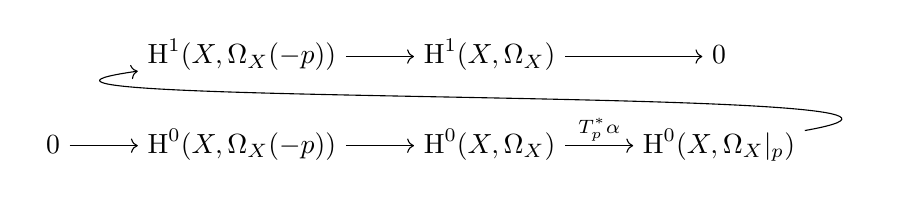
\begin{tikzpicture}[descr/.style={fill=white,inner sep=1.5pt}]
        \matrix (m) [
            matrix of math nodes,
            row sep=1.8em,
            column sep=2.5em,
            text height=1.5ex, text depth=0.25ex
        ]
        {  & \Hnm^1(X, \Omega_X(-p)) &  \Hnm^1(X, \Omega_X) & 0 &  \\
          0  & \Hnm^0(X, \Omega_X(-p)) & \Hnm^0(X, \Omega_X) & \Hnm^0(X, \Omega_X|_p) &  \\
        };

        \path[overlay,->, font=\scriptsize]
        
        (m-1-2) edge (m-1-3)
        (m-1-3) edge (m-1-4)
        (m-2-4) edge[out=10,in=188] (m-1-2)
        (m-2-1) edge (m-2-2)
        (m-2-2) edge (m-2-3)
        (m-2-3) edge node[above, yshift=-2pt] {$T_p^* \alpha$} (m-2-4)
        ;
\end{tikzpicture}
\end{center}
The proposition below follows from standard arguments in homological algebra:

\begin{proposition}\label{prop:dim_of_Albanese_image}
For a general point $p \in X$,
\begin{equation*}
\begin{aligned}
 \dim_{\mathbb{C}} \alpha(X) =\;& \rank T_p^* \alpha  \\ 
 =\;& n-h^0(X, \Omega_X(-p))  \\ 
 =\;& h^1(X, \Omega_X(-p))-h^1(X, \Omega_X).  \\ 
\end{aligned}
\end{equation*}
In particular,
\begin{equation*}
\begin{aligned}
  & \alpha \text{ is surjective} & \Longleftrightarrow\quad& h^0(X, \Omega_X(-p))=0 \\ 
  & \alpha \text{ is finite onto image} & \Longleftrightarrow\quad& h^0(X, \Omega_X(-p))=n-r \\ 
  & \alpha \text{ is constant} & \Longleftrightarrow\quad& h^0(X, \Omega_X(-p))=n \\ 
  & & \Longleftrightarrow\quad& h^1(X, \Omega_X(-p))=h^1(X, \Omega_X) \\ 
  & & \Longleftrightarrow\quad& n=0. \\ 
\end{aligned}
\end{equation*}
\end{proposition}
We will concentrate on the case where $\alpha$ is finite onto its image.\footnote{The general method remains valid in the broader setting, but the Gauss map then takes values in a different space.} Under this assumption, we set $Z = X$ and $A = \Alb(Z)$. The corresponding Gauss map is then a rational map:
% https://q.uiver.app/#q=WzAsNixbMCwwLCJcXHBoaV9aOiJdLFsyLDAsIlxcR3IocixUXjBBKSJdLFsxLDAsIloiXSxbMywwLCJcXEdyKG4tcixcXEhubV4wKFgsXFxPbWVnYV9YKSkiXSxbMywxLCJcXEhubV4wKFgsXFxPbWVnYV9YKC1wKSkiXSxbMSwxLCJwIl0sWzUsNCwiIiwwLHsic3R5bGUiOnsidGFpbCI6eyJuYW1lIjoibWFwcyB0byJ9fX1dLFsyLDEsIiIsMCx7InN0eWxlIjp7ImJvZHkiOnsibmFtZSI6ImRhc2hlZCJ9fX1dLFsxLDMsIlxcY29uZyIsMSx7InN0eWxlIjp7ImJvZHkiOnsibmFtZSI6Im5vbmUifSwiaGVhZCI6eyJuYW1lIjoibm9uZSJ9fX1dXQ==
\[\begin{tikzcd}[row sep={-1mm}]
	{\phi_Z:} &[-10mm] Z &[5mm] {\Gr(r,T^0A)} & [-7mm] {\Gr(n-r,\Hnm^0(X,\Omega_X))} \\
	& p && {\Hnm^0(X,\Omega_X(-p))}
	\arrow[dashed, from=1-2, to=1-3]
	\arrow["\cong"{description}, draw=none, from=1-3, to=1-4]
	\arrow[maps to, from=2-2, to=2-4]
\end{tikzcd}\]
and we have the isomorphisms 
\begin{equation*}
\begin{aligned}
   \mathbb{P}T^{*}_{0}A \cong\;& \mathbb{P}\Hnm^0(X,\Omega_X), \\ 
    \mathbb{P}\Lambda_{Z}=\;& \left\{\, (p,[\omega])  \in Z \times \mathbb{P}T^{*}_{0}A \;\middle|\; \omega(p)=0 \,\right\}  \\ 
    \cong\;& \left\{\,\rule{0mm}{3.2mm} (p,[\omega])  \in Z \times \mathbb{P}T^{*}_{0}A \;\middle|\; \omega \in \Hnm^0(X,\Omega_X(-p)) \,\right\}  \\ 
    \cong\;& \left(\phi_Z, \Id \right)^{-1} I_{n-r, 1},  \\ 
\end{aligned}
\end{equation*}
where 
$$I_{n-r, 1}:= \left\{\, \rule{0mm}{3.2mm} (V,[\omega])  \in \Gr(n-r,n) \times \Gr(1, n) \;\middle|\; \omega \in V \,\right\}$$ 
is the incidence variety relating $\Gr(n-r,n)$ and $\Gr(1, n)$. In that case, 
\begin{equation*}
\begin{aligned}
    \gamma_Z^{-1}([\omega])=\;& \left\{\, p  \in X  \;\middle|\; \omega(p)=0 \,\right\}  \\  
\end{aligned}
\end{equation*}
is the zero set of section $\omega \in \Hnm^0(X,\Omega_X)$. The number $(-1)^r \deg \gamma_Z$ is the index in the Poincaré--Hopf index formula, and the monodromy group $\Gal(\gamma_Z)$ serves as a more refined invariant, encoding subtler aspects of the geometry.

The next proposition shows when the Gauss map $\phi_Z$ is not generic injective.
\begin{proposition}
When $\alpha$ is finite onto its image,
\begin{equation*}
\begin{aligned}
  \;&  \phi_Z \text{ is not generic injective} \\ 
  \Longleftrightarrow\;\;& \text{For general $p \in X$, exists $q \neq p$ such that $h^0(X,\Omega_X(-p-q))=n-r$} \\ 
  \stackrel{\textcolor{purple}{\textbf{?}\footnotemark}}{\Longleftrightarrow}\;\;& \text{For general $p \in X$, exists $S \in X^{[2]}$ such that $p\in S$ and $h^0(X,\Omega_X \otimes \mathcal{I}_S)=n-r$} \\ 
  \Longleftrightarrow\;\;& \text{For all $p \in X$, exists $S \in X^{[2]}$ such that $p\in S$ and $h^0(X,\Omega_X \otimes \mathcal{I}_S)\geqslant n-r$.} \\ 
\end{aligned}
\end{equation*}
\end{proposition}
\footnotetext{When $n = r$, the map $\varphi_Z$ has a point as its target, so the equivalence is trivial.
When $n > r$, the implication ``$\Rightarrow$" is immediate. For the converse ``$\Leftarrow$", it suffices to show that the image of 
$$\left\{ S \in X^{[2]} \;\middle|\; h^0(X,\Omega_X \otimes \mathcal{I}_S)=n-r   \right\}$$
 under the map $\pi_X:X^{[2]} \longrightarrow X^{(2)} $ does not include the diagonal. Indeed, we can choose a section $s \in \Hnm^0(X,\Omega_X)$ that cuts out finitely many reduced points $p_1,\ldots,p_d$ in $X$. (Well this maybe not so true, since $\phi_Z$ is not always regular, such a section $s$ may vanish along some indeterminacy locus. However, for a general $s$, there will always be at least one isolated zero $p_1$, which is sufficient for our purposes.)
Then for any $S \in \pi_X^{-1}(p_1)$, we have 
$$\Hnm^0(X,\Omega_X \otimes \mathcal{I}_S)  \subsetneqq \Hnm^0(X,\Omega_X(-p_1)).$$
}
This last step relies on the following lemma, combined with the closedness of the tautological correspondence in $X \times X^{[2]}$.
\begin{lemma}
Let $m \in \mathbb{Z}_{>0}$. The function $$h^{\Omega}: X^{[m]} \longrightarrow \mathbb{Z}_{\geqslant 0} \qquad
 S \longmapsto h^0(X,\Omega_X \otimes \mathcal{I}_S)$$ 
is Zariski upper semicontinuous.
\end{lemma}
\begin{proofsketch}
Consider the coherent sheaf $\mathcal{F} \in \Coh(X^{[m]} \times X)$ characterized by the property
$$\mathcal{F}|_{\{S\} \times X} \cong \Omega_X \otimes \mathcal{I}_S,$$
The proposition then follows directly from the semicontinuity theorem \cite[28.1.1]{vakil2017rising}.
\end{proofsketch}

The stratification of $X^{[m]}$ by $h^{\Omega}$ offers a natural generalization of Brill--Noether theory beyond the setting of curves.

$\,$

At the end of this subsection, let us turn to the setting of a general abelian variety $A$ and a smooth subvariety $\iota_Z: Z \hookrightarrow A$, where $n = \dim_{\mathbb{C}} A$ and $r = \dim_{\mathbb{C}} Z$. Observe that $\iota_Z$ factors through the Albanese variety of $Z$:
% https://q.uiver.app/#q=WzAsMyxbMCwwLCJcXGlvdGFfWjogWiAgIl0sWzEsMCwiXFxBbGIoWikiXSxbMiwwLCJBIl0sWzAsMSwiXFxhbHBoYV9aIl0sWzEsMiwiXFxwaSJdXQ==
\[\begin{tikzcd}[column sep=large]
	{\iota_Z: Z  } & {\Alb(Z)} & A
	\arrow["{\alpha_Z}", from=1-1, to=1-2]
	\arrow["\pi", from=1-2, to=1-3]
\end{tikzcd}\]

We shall also assume that $Z$ generates $A$; it then follows that the map $\pi$ is surjective. The cotangent map of $\iota_Z$ at a point $p \in Z$ factors through $\Hnm^0(Z, \Omega_Z)$:
% https://q.uiver.app/#q=WzAsMyxbMCwwLCJUX3BeKiBcXGlvdGFfWjogVF9wXipBICAiXSxbMSwwLCJcXEhubV4wKFosIFxcT21lZ2FfWikiXSxbMiwwLCJUX3BeKloiXSxbMCwxLCIiLDAseyJzdHlsZSI6eyJ0YWlsIjp7Im5hbWUiOiJob29rIiwic2lkZSI6InRvcCJ9fX1dLFsxLDJdXQ==
\[\begin{tikzcd}[column sep=large]
	{T_p^* \iota_Z: T_p^*A  } & {\Hnm^0(Z, \Omega_Z)} & {T_p^*Z}
	\arrow[hook, from=1-1, to=1-2]
	\arrow[from=1-2, to=1-3]
\end{tikzcd}\]
For convenience, abbreviate $V := T_0^*A \cong T_p^*A$, and view $V$ as a subspace of $\Hnm^0(Z, \Omega_Z)$.
\begin{proposition}
Assume that $Z$ is embedded in $A$ and generates $A$, and let $V := T_0^*A$. Then
$$\dim_{\mathbb{C}} \Hnm^0(Z,\Omega_Z(-p)) \cap V =n-r \qquad \text{ for all $p \in Z$}$$
It follows that the Gauss map is a regular morphism
\[\begin{tikzcd}[row sep={-1mm}]
	{\phi_Z:} &[-10mm] Z &[5mm] {\Gr(r,T^0A)} & [-7mm] {\Gr(n-r,V)} \\
	& p && {\Hnm^0(Z,\Omega_Z(-p)) \cap V}
	\arrow[from=1-2, to=1-3]
	\arrow["\cong"{description}, draw=none, from=1-3, to=1-4]
	\arrow[maps to, from=2-2, to=2-4]
\end{tikzcd}\]
 Furthermore, 
\begin{equation*}
\begin{aligned}
  \;&  \phi_Z \text{ is not generic injective} \\ 
  \Longleftrightarrow\;\;& \text{For general $p \in Z$, exists $q \neq p$ such that $h^0(Z,\Omega_Z(-p-q)) \cap V =n-r$} \\ 
  \Longleftrightarrow\;\;& \text{For all $p \in Z$, exists $S \in Z^{[2]}$ such that $p\in S$ and $h^0(Z,\Omega_Z \otimes \mathcal{I}_S) \cap V=n-r$.} \\ 
\end{aligned}
\end{equation*}
\end{proposition}



\section{Families of subvarieties}\label{sec:subvarieties}

In this section, we move from the study of monodromy groups to a more direct analysis of the subvarieties themselves. Given an initial subvariety, one can naturally generate a family of subvarieties. Our goal here is to define these families and investigate their properties.

\subsection{Clean Lagrangian cycles}
\begin{proposition}
All irreducible conic Lagrangian cycles in $T^*A$ are of the form $\Lambda_Z$ for some irreducible subvariety $Z \subset A$. This yields a one-to-one correspondence between irreducible conic Lagrangian cycles in $T^*A$ and irreducible subvarieties of $A$:
$$\left\{\text{ irreducible conic Lagrangian cycles in $T^*A$ }   \right\} \longleftrightarrow \left\{\text{ irreducible subvarieties in $A$ }   \right\}$$
\end{proposition}

\begin{proofsketch}
For any irreducible conic Lagrangian cycle $\mathbf{\Lambda} \subset T^*A$, let $Z$ denote the image of $\mathbf{\Lambda}$ under the natural projection $T^*A \to A$. Our goal is to show that $\mathbf{\Lambda} = \Lambda_Z$.
\begin{itemize}
\item By definition, $\mathbf{\Lambda} \subset T^*A|_Z$.
\item Since $\mathbf{\Lambda}$ is conic, we have $s(Z) \subset \mathbf{\Lambda}$, where $s : A \to T^*A$ denotes the zero section.
\item Since $\mathbf{\Lambda}$ is Lagrangian and $s(Z) \subset \mathbf{\Lambda}$, we have $\mathbf{\Lambda} \subset \Lambda_Z$.
\item Since $\Lambda_Z$ is irreducible with $\dim_{\mathbb{C}} \mathbf{\Lambda} = \dim_{\mathbb{C}} \Lambda_Z = n$, we have $\mathbf{\Lambda} = \Lambda_Z$.
\end{itemize}
\end{proofsketch}

Why do we shift attention from $Z$ to $\Lambda_Z$ as the main object of study? One reason is the uniformity of $\Lambda_Z$: it always has dimension $n$, and in most cases, the natural map $\Lambda_Z \to T_0^* A$ is generically finite, with fibers lying inside $A$.

\begin{definition}[Clean cycle]
An irreducible Lagrangian cycle $\mathbf{\Lambda} \subset T^*A$ is called clean if the composed projection
$$\mathbf{\Lambda} \longrightarrow T^*A \twoheadrightarrow T_0^*A$$
is generically finite.
\end{definition}

Another important reason is that the space of weighted clean conic Lagrangian cycles naturally acquires a convolution structure, arising from the group law on $A$, which plays a central role in the analysis.

\begin{proposition}
The group of weighted clean conic Lagrangian cycles
\begin{equation*}
\begin{aligned}
  \mathcal{L}(A):=\;& \left\{ \text{weighted clean conic Lagrangian cycles in }T^*A \right\}  \\ 
  =\;& \left\{ \raisebox{1.5mm}{$\displaystyle\sum_{\substack{Z_i \subset A \\ \text{irr clean}}}$}n_i \Lambda_{Z_i}\; \middle|\; n_i \in \mathbb{Z} \right\}  \\ 
\end{aligned}
\end{equation*}
has a natural convolution structure as follows: 
\begin{equation*}
\begin{aligned}
  \Lambda_{Z_1} \circ \Lambda_{Z_2}=\;& \text{ the clean part of }(a,\Id_{T_0^* A})_* \left( \Lambda_{Z_1} \times_{T_0^* A} \Lambda_{Z_2} \right) \\ 
  =\;& \overline{(a,\Id_{U})_* \left( \Lambda_{Z_1}|_U \times_{U} \Lambda_{Z_2}|_U \right)} \\ 
\end{aligned}
\end{equation*}
where 
$$U:=\left\{ \xi \in T_0^*A \; \middle|\; \rule{0mm}{3.4mm}\deg \phi_{Z_i}= \# \phi_{Z_i}^{-1}(\xi) \text{ for } i=1,2 \right\}$$
and $a: A \times A \longrightarrow A$ is the addition map in $A$. The general convolution is defined by $\mathbb{Z}$-linear extension.
\end{proposition}

\begin{proofsketch}
To establish the claim, it suffices to show that $\Lambda_{Z_1} \circ \Lambda_{Z_2}$ defines a weighted conic Lagrangian cycle. The conic property follows directly from the definition, while the Lagrangian condition can be verified at a general point $(p_1 + p_2, \xi) \in \Lambda_{Z_1} \circ \Lambda_{Z_2}$.
\end{proofsketch}

We now consider the projective versions of all objects involved, so that we may make use of properness. To simplify notation, we abbreviate $\mathbb{P}T^{*}_{0}A$ by $\mathbb{P}^{\vee}$.

\begin{lemma}\label{lem:mon_of_prod}\
\begingroup
\upshape
%\setlist{itemsep=-0.4em}
\renewcommand\labelenumi{(\theenumi)}
\begin{enumerate}[(1)]
\item Suppose that $\mathbb{P}\Lambda_{Z_1}, \mathbb{P}\Lambda_{Z_1} \subset \mathbb{P}T^*A$ admit monodromy representations $$\rho_{\gamma_{Z_i}}: \pi_1(U,\xi_0) \longrightarrow \Aut\left(\gamma_{Z_i}^{-1}(\xi_0)\right),$$ 
then $\mathbb{P}\Lambda_{Z_1} \times_{\mathbb{P}^{\vee}} \mathbb{P}\Lambda_{Z_2} \subset A\times A \times \mathbb{P}^{\vee}$ admits monodromy representation given by
$$(\rho_{\gamma_{Z_1}},\rho_{\gamma_{Z_2}}): \pi_1(U,\xi_0) \longrightarrow \Aut\left(\gamma_{Z_1}^{-1}(\xi_0) \times \gamma_{Z_2}^{-1}(\xi_0)\right),$$ 
\item When $Z_1=Z_2=Z$, we obtain an one-to-one correspondence:
$$\left\{ 
\begin{aligned}
  &\text{ irr components of } \mathbb{P}\Lambda_{Z} \times_{\mathbb{P}^{\vee}} \mathbb{P}\Lambda_{Z}  \\ 
  &\hspace{10mm}\text{ with a surjection to } \mathbb{P}^{\vee}
\end{aligned}
 \right\} \longleftrightarrow 
\left\{ 
\begin{aligned}
  &\Gal(\gamma_{Z})\text{-orbits of }  \\ 
  &\;\;\gamma_{Z}^{-1}(\xi_0) \times \gamma_{Z}^{-1}(\xi_0)
\end{aligned}
 \right\} 
 $$
\end{enumerate}
\endgroup
\end{lemma}
\begin{proofsketch}
Statement (1) holds by definition. The proof of (2) reduces to the following purely topological statement:
\begin{claim}
Let $\pi: E \longrightarrow B$ be a (unramified) covering space over a manifold $B$ with deck transformation group $G$, then
$$\left\{ \rule{0mm}{3.1mm}\text{ connected components of }E \times_B E \;\right\} \longleftrightarrow \left\{   \;G\text{-orbits of } \pi^{-1}(b_0) \times \pi^{-1}(b_0)\; \right\}. $$
\end{claim}
\noindent The claim follows directly from the correspondence between covering spaces over $B$ and $\pi_1(B)$-sets; see \cite[Theorem 1.38]{Ha02}.
\end{proofsketch}

Generalizing the argument of Lemma \ref{lem:mon_of_prod}, we arrive at the following lemma.

\begin{lemma}
For $d=\deg \gamma_{Z}$, $\xi_0 \in T_0^* A$ a general point, write
\begin{equation*}
\begin{aligned}
  \mathbb{P}\Lambda_{Z}^{\times d} :=\;&\;\; \mathbb{P}\Lambda_{Z} \times_{\mathbb{P}^{\vee}}\mathbb{P}\Lambda_{Z} \times_{\mathbb{P}^{\vee}} \cdots \times_{\mathbb{P}^{\vee}} \mathbb{P}\Lambda_{Z} && \subset A^d \times \mathbb{P}^{\vee}\\ 
  \gamma_{Z}^{-1}(\xi_0)^{d} :=\;& \gamma_{Z}^{-1}(\xi_0) \times \gamma_{Z}^{-1}(\xi_0) \times \cdots \times \gamma_{Z}^{-1}(\xi_0) && \subset A^d \\ 
\end{aligned}
\end{equation*}
\begingroup
\upshape
%\setlist{itemsep=-0.4em}
\renewcommand\labelenumi{(\theenumi)}
\begin{enumerate}[(1)]
\item we obtain an one-to-one correspondence:
$$\left\{ 
\begin{aligned}
  &\text{ irr components of } \mathbb{P}\Lambda_{Z}^{\times d}  \\ 
  &\hspace{0mm}\text{ with a surjection to } \mathbb{P}^{\vee}
\end{aligned}
 \right\} \longleftrightarrow 
\left\{ 
\begin{aligned}
  &\Gal(\gamma_{Z})\text{-orbits of }  \\ 
  &\hspace{8mm}\gamma_{Z}^{-1}(\xi_0) ^d
\end{aligned}
 \right\} 
 $$
\item Write
\begin{equation*}
\begin{aligned}
  \Delta_d :=\;&\left\{ (p_1,\ldots,p_d) \in A^d \;\middle|\; p_i=p_j \text{ for some } i \neq j  \right\} && \subset A^d \\ 
  \mathbb{P}\Lambda_{Z}^{[d]} :=\;& \overline{\left( \mathbb{P}\Lambda_{Z}^{\times d} \smallsetminus \left( \Delta_d \times \mathbb{P}^{\vee} \right) \right)|_U} && \subset A^d \times \mathbb{P}^{\vee}\\ 
\end{aligned}
\end{equation*}
Fix a general point $\xi_0 \in \mathbb{P}^{\vee}$ and a well-order for $\gamma_{Z}^{-1}(\xi_0)$, one can identify $S_d \cong \gamma_{Z}^{-1}(\xi_0)^d \smallsetminus \Delta_d$, and 
$$\left\{ 
\text{ irr components of } \mathbb{P}\Lambda_{Z}^{[d]}  
 \;\right\} \longleftrightarrow 
\left\{ \;\rule{0mm}{3.3mm}
\Gal(\gamma_{Z})\text{-orbits of }  S_d
 \;\right\} 
 $$
 In reference, $\Delta_d$ is usually called the big diagonal.
\end{enumerate}
\endgroup
\end{lemma}

From this point on, we fix an irreducible component of $\mathbb{P}\Lambda_{Z}^{[d]}$, denoted by $\mathbb{P}\Lambda_{Z}^{\univ}$. As we will see in Definition \ref{def:subvar_Z^{(m)}}, this variety generates all subvarieties within the families under consideration.

\begin{definition}[The subvariety $Z^{(m)}$]\label{def:subvar_Z^{(m)}}
For any tuple $(m) = (m_1, \ldots, m_d) \in \mathbb{Z}^d$, we define the weighted sum map
$$a^{(m)}: A^d \longrightarrow A \qquad (p_1,\ldots,p_d) \longmapsto \sum_{i=1}^{d} m_ip_i.$$
We also define 
$$\mathbb{P}\Lambda_{Z}^{(m)}: = \left( a^{(m)},\Id_{\mathbb{P}^{\vee}}  \right)_* \mathbb{P}\Lambda_{Z}^{\univ}.$$
as the (projectivized) weighted Lagrangian cycle in $\mathbb{P}T^*A$. The projective cycle $\mathbb{P}\Lambda_{Z}^{(m)}$ is irreducible but may appear with multiplicities. We can therefore write
$$\mathbb{P}\Lambda_{Z}^{(m)} = c_Z^{(m)}  \mathbb{P}\Lambda_{Z^{(m)}}$$
where $c_Z^{(m)} \in \mathbb{Z}_{>0}$ and $Z^{(m)} \subset A$ are uniquely determined. This gives rise to a family of subvarieties parametrized by $\mathbb{Z}^d$.
\end{definition}

The next lemma gathers some basic properties of $Z^{(m)}$. Observe that $S_d=\Aut\left(\gamma_{Z}^{-1}(\xi_0)\right)$ acts naturally on $\mathbb{Z}^d$ via
$$g(m)=\left(m_{g(1)},\ldots , m_{g(d)}\right) \in \mathbb{Z}^d.$$

\begin{lemma}\
\begingroup
\upshape
%\setlist{itemsep=-0.4em}
\renewcommand\labelenumi{(\theenumi)}
\begin{enumerate}[(1)]
\item For all $g\in \Gal(\gamma_{Z})$, we have $ Z^{g(m)}=Z^{(m)}$, $c_Z^{g(m)}=c_Z^{(m)}$;
\item For $(m)=(1,0,\ldots,0)\in \mathbb{Z}^d$, $Z^{(m)}=Z$;
\item For all $(m), (m') \in \mathbb{Z}^d$, we have  $\mathbb{P}\Lambda_{Z}^{(m)} \circ \mathbb{P}\Lambda_{Z}^{(m')} \supseteq \mathbb{P}\Lambda_{Z}^{(m+m')}$;
\item The group $\left< \mathbb{P}\Lambda_{Z^{(m)}} \right>_{\Abel}$ is closed under the convolution product.
\end{enumerate}
\endgroup
\end{lemma}

\subsection{Realized as characteristic cycles}\label{subsec:relation_with_perverse_sheaf}

In fact, the Lagrangian cycles $\mathbb{P}\Lambda_{Z^{(m)}}$ coincide with the irreducible components of the clean cycles described in \cite[2.c]{Kr20} and \cite[p5, Theorem 1.7]{Kr22GaussI}, leading to the following relations:
% https://q.uiver.app/#q=WzAsNixbMCwwLCJcXFBlcnYoQSkvTihBKSJdLFsxLDAsIlxcbGVmdDwgXFxkZWx0YV9aIFxccmlnaHQ+Il0sWzIsMCwiXFxSZXAgXFxsZWZ0KFxccnVsZXswbW19ezNtbX1HX3VcXHJpZ2h0KSJdLFswLDEsIlxcbWF0aGNhbHtMfShBKSJdLFsxLDEsIlxcbGVmdDwgXFxjaGFyY3ljbGUoXFxkZWx0YV9aKSBcXHJpZ2h0PiJdLFsyLDEsIlxcUmVwIFxcbGVmdChcXHJ1bGV7MG1tfXszbW19VF91IFxccnRpbWVzIFxcR2FsKFxcZ2FtbWFfWilcXHJpZ2h0KSJdLFsxLDAsIlxcc3Vwc2V0IiwxLHsic3R5bGUiOnsiYm9keSI6eyJuYW1lIjoibm9uZSJ9LCJoZWFkIjp7Im5hbWUiOiJub25lIn19fV0sWzEsNCwiXFxjaGFyY3ljbGUiXSxbMSwyLCJcXGNvbmciLDEseyJzdHlsZSI6eyJib2R5Ijp7Im5hbWUiOiJub25lIn0sImhlYWQiOnsibmFtZSI6Im5vbmUifX19XSxbMiw1XSxbNCw1LCJcXHN0YWNrcmVsez99e1xcY29uZ30iLDEseyJvZmZzZXQiOi0xLCJzdHlsZSI6eyJib2R5Ijp7Im5hbWUiOiJub25lIn0sImhlYWQiOnsibmFtZSI6Im5vbmUifX19XSxbNCwzLCJcXHN1cHNldCIsMSx7InN0eWxlIjp7ImJvZHkiOnsibmFtZSI6Im5vbmUifSwiaGVhZCI6eyJuYW1lIjoibm9uZSJ9fX1dXQ==
\[\begin{tikzcd}[column sep=5mm,row sep=5mm]
	{\Perv(A)/N(A)} & {\left< \delta_Z \right>} & {\Rep \left(\rule{0mm}{3mm}G_u\right)} \\
	{\hspace{14mm}\mathcal{L}(A)} & {\left< \charcycle(\delta_Z) \right>} & {\Rep \left(\rule{0mm}{3mm}T_u \rtimes \Gal(\gamma_Z)\right)}
	\arrow["\supset"{description}, draw=none, from=1-2, to=1-1]
	\arrow["\cong"{description}, draw=none, from=1-2, to=1-3]
	\arrow["\charcycle", from=1-2, to=2-2]
	\arrow[from=1-3, to=2-3]
	\arrow["\supset"{description}, draw=none, from=2-2, to=2-1]
	\arrow["{\stackrel{\footnotemark}{\cong}}"{description}, shift left, draw=none, from=2-2, to=2-3]
\end{tikzcd}\]
\footnotetext{I believe that this isomorphism should be already known, so I should probably cite it somewhere(rather than making it up all by myself).}
Here, $\delta_Z$ denotes the perverse intersection complex associated with the subvariety $Z$ (in particular, $\delta_Z = \iota_{Z,*}\underline{\mathbb{Q}}_Z[-\dim Z]$ when $Z$ is smooth), and $\mathcal{L}(A)$ stands for the $\lambda$-ring of clean conic Lagrangian cycles on $T^*A$ \cite[p5]{Kr21GaussII}.

\begin{remark}
Suppose that $Z \subset A$ is smooth of general type. Then the characteristic cycle $\charcycle(\delta_Z)$ is irreducible and equals $\mathbb{P}\Lambda_Z$. In this situation, let ${\lambda_1, \ldots, \lambda_d} \subset X^*(T_u)$ denote the weights corresponding to the points $p_1, \ldots, p_d \in \gamma_Z^{-1}(\xi_0)$.
For each tuple $(m) \in \mathbb{Z}^d$, define $\lambda^{(m)} = \sum m_i \lambda_i \in X^*(T_u)$, and consider the ``highest weight representation"
$$V_{\lambda^{(m)}}=\bigoplus_{\lambda \in \Gal(\gamma_{Z}) \cdot \lambda^{(m)}} \mathbb{C}_{\lambda} \in \Rep
\left(\rule{0mm}{3mm}T_u \rtimes \Gal(\gamma_Z)\right)$$
where $\mathbb{C}_\lambda$ is the one-dimensional representation of $T_u$ with weight $\lambda$. Under this correspondence, one has an explicit identification
$$\left< \mathbb{P}\Lambda_{Z} \right> \cong \Rep
\left(\rule{0mm}{3mm}T_u \rtimes \Gal(\gamma_Z)\right) \qquad \mathbb{P}\Lambda_{Z^{(m)}} \longleftrightarrow V_{\lambda^{(m)}}.$$

Moreover, the Weyl group $W_Z$ acts naturally on $X^(T)$. For the orbit $W_Z \cdot \chi_0 \subset X^(T)$, the associated Lagrangian cycle is given by
$$\sum_{\sigma \in W_Z/\Gal(\gamma_Z)} \mathbb{P}\Lambda_{Z^{\sigma (\chi_0)}}.$$


\end{remark}

\section{Monodromy group}\label{sec:mon_examples}

\subsection{Curves in Prym variety with small monodromy group}\label{subsec:small_mon}
This subsection is devoted to presenting an example that has small monodromy group.


\begin{setting}\label{set:Prym}
Suppose $C'$ is a smooth projective curve of genus $g(C')$, and let $B$ be an effective (possibly zero) divisor on $C'$. For any line bundle $\eta \in \Pic(C')$ such that $\eta^{\otimes 2} \cong \mathcal{O}_{C'}(B)$, one obtains a double cover $h: C \to C'$ of smooth projective curves, ramified precisely over $B$. The associated involution on $C$ is denoted by $\iota$, and the triple $(C, C', h)$ is referred to as the Prym pair.

Recall that the Prym variety $A := \Prym(C/C')$ is defined as the connected component of the identity in 
$$\ker \left[\Nm:\rule{0mm}{3.4mm}\Jac(C) \longrightarrow \Jac(C') \right].$$ 
The Abel--Prym map is defined by
$$\AP_{C/C'}: C \longrightarrow A \qquad p \longmapsto \mathcal{O}_{C}(p-\iota(p)).$$
\end{setting}

The classical theory treats the case where the Prym variety $A$ is principally polarized—this occurs exactly when $B = \varnothing$ or $B =\{p_0, q_0\}$, that is, when $h$ is either unramified or ramified at two points.\footnote{See \cite[Theorem 3.2.6]{CK22} for the proof.} For clarity, we restrict our attention to these cases. Table \ref{table:Prym_numerical_data} lists the relevant numerical data.\footnote{As usual, $n=\dim_{\mathbb{C}} A$ is the dimension of the abelian variety.}

{
\def\arraystretch{1.2}
\begin{table}[ht]
\begin{tabular}{c|c|c|c}
\hline
                  & $g(C)$ & $g(C')$ & $\deg \eta$ \\ \hline
$B = \varnothing$ & $2n+1$ & $n+1$   & $0$         \\ \hline
$B =\{p_0, q_0\}$ & $2n$   & $n$     & $1$         \\ \hline
\end{tabular}
\medskip
\caption{numerical data of Prym pair}
\label{table:Prym_numerical_data}
\vspace*{-\baselineskip}
\end{table}
}
The Abel–Prym map $\AP_{C/C'}$ does not always behave as nicely as the Abel–Jacobi map; it may fail to be an embedding. When $C$ is hyperelliptic, the map $\AP_{C/C'}$ fails to be generically injective, and therefore falls outside the scope of our discussion. When $C$ is non-hyperelliptic, we may regard it as a subvariety of $A$ for our purposes, although it may be not strictly embedded.\footnote{For a detailed description of the map $\AP_{C/C'}$, see \cite[Proposition 12.5.2, Corollary 12.5.6]{BL04}. Although $\AP_{C/C'}$ may collapse $p_0$ and $q_0$, this does not affect the relevant computation of $\Gal(\gamma_Z)$.} However, it remains unclear whether $C$ is stable under any translation in $A$.

In the Prym setting, the corresponding Gauss map $\gamma_C$ factors through $h$: 
% https://q.uiver.app/#q=WzAsMTEsWzAsMCwiXFxnYW1tYV9DOiJdLFsxLDAsIkMiXSxbMiwwLCJDJyJdLFszLDAsIlxcbWF0aGJie1B9XntuLTF9Il0sWzUsMCwiXFxtYXRoYmJ7UH1cXCFcXGxlZnQoIEheMChcXG9tZWdhX3tDJ30gXFxvdGltZXMgXFxldGEpXiogXFxyaWdodCkiXSxbNSwxLCJcXEdyXFxsZWZ0KG4tMSwgSF4wKFxcb21lZ2Ffe0MnfSBcXG90aW1lcyBcXGV0YSlcXHJpZ2h0KSJdLFs1LDIsIkheMFxcbGVmdChcXG9tZWdhX3tDJ30gXFxvdGltZXMgXFxldGEoLXApXFxyaWdodCkiXSxbMiwyLCJwIl0sWzEsMiwiXFx0aWxkZXtwfSJdLFs0LDAsIj0iXSxbNCwxLCJcXGNvbmciXSxbOCw3LCIiLDAseyJzdHlsZSI6eyJ0YWlsIjp7Im5hbWUiOiJtYXBzIHRvIn19fV0sWzIsMywifFxcb21lZ2Ffe0MnfSBcXG90aW1lcyBcXGV0YXwiXSxbMSwyLCJoIl0sWzcsNiwiIiwwLHsic3R5bGUiOnsidGFpbCI6eyJuYW1lIjoibWFwcyB0byJ9fX1dXQ==
\[\begin{tikzcd}[column sep=10mm,row sep=-2mm]
	{\gamma_C:} &[-12mm] C & {C'} & [5mm] {\mathbb{P}^{n-1}} & [-12mm]{=} &[-12mm] {\hspace{-10mm}\mathbb{P}\!\left( \Hnm^0(\omega_{C'} \otimes \eta)^* \right)} \\
	&&&& \cong & {\Gr\left(n-1, \Hnm^0(\omega_{C'} \otimes \eta)\right)} \\[1mm]
	& {\tilde{p}} & p &&& {\Hnm^0\left(\omega_{C'} \otimes \eta(-p)\right)}
	\arrow["h", from=1-2, to=1-3]
	\arrow["{|\omega_{C'} \otimes \eta|}", from=1-3, to=1-4]
	\arrow[maps to, from=3-2, to=3-3]
	\arrow[maps to, from=3-3, to=3-6]
\end{tikzcd}\]


\begin{eg} \label{eg:bielliptic}
Let $C'$ be a non-hyperelliptic bielliptic curve, and let $\pr: C' \to E$ denote a $2:1$ covering onto an elliptic curve. For any nontrivial $2$-torsion line bundle $\eta_0 \in \Pic^0(E)[2]$, the pullback $\eta := \pr^* \eta_0$ satisfies $\eta^{\otimes 2} \cong \mathcal{O}_{C'}$ and the map $|\omega_{C'} \otimes \eta|$ factors through $\pr$.
\end{eg}
\begin{proof}[{Proof of Example \ref{eg:bielliptic}}]
For any $x \in C'$, write $x_0:= \pr(x)$, then
$$ \deg \eta_0^{\vee} (x_0)=1 \quad \Longrightarrow \quad \text{ there exists } y_0 \in E \text{ such that } \eta_0^{\vee} (x_0)=\mathcal{O}_E(y_0).$$
Write $\pr^{-1}(x_0)=\{x,x'\}$, $\pr^{-1}(y_0)=\{y,y'\}$, we get
\begin{equation*}
\begin{aligned}
\;& \eta_0^{\vee} (x_0)=\mathcal{O}_E(y_0) && \\ 
\Longrightarrow\;& \eta^{\vee}(x+x')= \mathcal{O}_{C'}(y+y') && \text{Via pulling back along $\pr$} \\ 
  \Longrightarrow\;& h^0 \left(\rule{0mm}{3mm} \eta^{\vee}(x+x')\right) = 1 && \\ 
  \Longleftrightarrow\;& h^0 \left(\rule{0mm}{3mm}\omega_{C'} \otimes \eta(-x-x')\right) = n - 1 && \text{Via Riemann--Roch}\\
  \Longleftrightarrow\;& \Hnm^0 \left(\rule{0mm}{3mm}\omega_{C'} \otimes \eta(-x)\right) \cong  \Hnm^0 \left(\rule{0mm}{3mm}\omega_{C'} \otimes \eta(-x')\right) \qquad && \\ 
  \Longleftrightarrow\;& |\omega_{C'} \otimes \eta|(x)=|\omega_{C'} \otimes \eta|(x') &&
\end{aligned}
\end{equation*}
\end{proof}

The next proposition tells us, if we put some Galois condition for the covering, then the resulting curve $C \subset A$ is not invariant under any non-trivial translation of $A$. 

\begin{proposition}\label{prop:Galois_condition}
In Example \ref{eg:bielliptic}, let $C$ be the curve corresponding to $\eta \in \Pic^{0}(C')[2]$. If $\Gal(C/E) \cong \mathbb{Z}/2\mathbb{Z} \oplus \mathbb{Z}/2\mathbb{Z}$, then $C$ admits three intermediate quotients over $E$. Denote them by $C'$, $C_1$, and $C_2$, where $C_1$ and $C_2$ are the two intermediate curves different from $C'$.

% https://q.uiver.app/#q=WzAsMTIsWzAsMCwiQyJdLFswLDEsIkMnIl0sWzIsMCwiQyJdLFsyLDEsIkMnIl0sWzIsMiwiRSJdLFsyLDMsIlxcbWF0aGJie1B9XjEiXSxbMCwyLCJFIl0sWzAsMywiXFxtYXRoYmJ7UH1eMSJdLFsxLDEsIkNfMSJdLFszLDEsIkNfMiJdLFsyLDQsIlxcR2FsKEMvRSkgXFxjb25nIFxcbWF0aGJie1p9LzJcXG1hdGhiYntafSBcXG9wbHVzIFxcbWF0aGJie1p9LzJcXG1hdGhiYntafSJdLFswLDQsIlxcR2FsKEMvRSkgXFxjb25nIFxcbWF0aGJie1p9LzRcXG1hdGhiYntafSJdLFsxLDZdLFswLDEsImgiXSxbNiw3XSxbMiwzLCJoIl0sWzMsNF0sWzQsNV0sWzgsNF0sWzksNF0sWzIsOSwiaF8yIl0sWzIsOCwiaF8xIiwyXV0=
\[\begin{tikzcd}[ampersand replacement=\&,column sep={10mm,between origins},row sep=5mm]
	C \&[30mm]\&[2mm] C \\
	{C'} \& {C_1} \& {C'} \& {C_2} \\
	E \&\& E \\
	{\mathbb{P}^1} \&\& {\mathbb{P}^1} \\[-3mm]
	{\Gal(C/E) \cong \mathbb{Z}/4\mathbb{Z}} \&\& {\Gal(C/E) \cong \mathbb{Z}/2\mathbb{Z} \oplus \mathbb{Z}/2\mathbb{Z}}
	\arrow["h", from=1-1, to=2-1]
	\arrow["{h_1}"', from=1-3, to=2-2]
	\arrow["h", from=1-3, to=2-3]
	\arrow["{h_2}", from=1-3, to=2-4]
	\arrow[from=2-1, to=3-1]
	\arrow[from=2-2, to=3-3]
	\arrow[from=2-3, to=3-3]
	\arrow[from=2-4, to=3-3]
	\arrow[from=3-1, to=4-1]
	\arrow[from=3-3, to=4-3]
\end{tikzcd}\]
If either $\Gal(C/E) \cong \mathbb{Z}/4\mathbb{Z}$, or $\Gal(C/E) \cong \mathbb{Z}/2\mathbb{Z} \oplus \mathbb{Z}/2\mathbb{Z}$ with the coverings $h_i:C \to C_i$ ramified, then the curve $C \subset A$ is not fixed under any non-trivial translation on $A$.
\end{proposition}

\begin{proof}
We prove by contradiction.
Assume there exists a non-trivial translation $\sigma:A\to A$ preserving $C$. Then the restriction $\sigma|_{C}:C \to C$ is an automorphism, and the induced map
$$h_{\sigma}: C \longrightarrow C/\sigma$$
is an unramified double covering. Since $\sigma$ is a translation, the Gauss map $\gamma_C$ necessarily factors through $h_{\sigma}$:
% https://q.uiver.app/#q=WzAsNixbMCwwLCJcXGdhbW1hX0PvvJoiXSxbMSwwLCJDIl0sWzIsMCwiQyciXSxbMywwLCJFIl0sWzQsMCwiXFxtYXRoYmJ7UH1ee24tMX0iXSxbMiwxLCJDL1xcc2lnbWEiXSxbMSwyLCIyOjEiXSxbMiwzLCIyOjEiXSxbMyw0LCJcXHN1YnNldCIsMSx7InN0eWxlIjp7ImJvZHkiOnsibmFtZSI6Im5vbmUifSwiaGVhZCI6eyJuYW1lIjoibm9uZSJ9fX1dLFsxLDUsImhfe1xcc2lnbWF9IiwyXSxbNSwzLCJcXGV4aXN0cyEiLDIseyJzdHlsZSI6eyJib2R5Ijp7Im5hbWUiOiJkYXNoZWQifX19XV0=
\[\begin{tikzcd}[ampersand replacement=\&,column sep=15mm,row sep=5mm]
	{\gamma_C:} \&[-17mm] C \& {C'} \& E \&[-13mm] {\mathbb{P}^{n-1}} \\
	\&\& {C/\sigma}
	\arrow["{2:1}", from=1-2, to=1-3]
	\arrow["{h_{\sigma}}"', from=1-2, to=2-3]
	\arrow["{2:1}", from=1-3, to=1-4]
	\arrow["\subset"{description}, draw=none, from=1-4, to=1-5]
	\arrow["{\exists!}"', dashed, from=2-3, to=1-4]
\end{tikzcd}\]
Without loss of generality, we may assume that $\deg(h_\sigma)=2$. By assumption, $C/\sigma$ coincides with $C'$, and $\sigma|_C$ is the involution $\iota$ associated with the cover $h:C\to C'$, which extends to an involution $\tilde\iota$ of $A$. According to \cite[Proposition 12.4.2]{BL04}, $\tilde\iota$ is a reflection. Hence $\sigma \circ \tilde\iota^{-1}$ is another reflection fixing $C$, which is impossible.

\end{proof}

%Maybe I should check \cite{CMS21,JC92} for more information on Prym varieties of bielliptic curves.

Unfortunately, the condition in Proposition \ref{prop:Galois_condition} is never met, and consequently the curve $C \subset A$ is preserved by a $2$-torsion translation of $A$, as explained below.

\begin{lemma}\label{lem:small_mon_but_translation_invariant}
In Example \ref{eg:bielliptic}, let $(\mathcal{L}_3,  \mathcal{L}_3^{\otimes 2} \cong \mathcal{O}_E(R))$ denote the line bundle associated with the double cover $C' \to E$, where $R$ is its branch divisor. Set $\mathcal{L}_1 := \eta_0$, $\mathcal{L}_2 := \eta_0 \otimes \mathcal{L}_3$, and let $u_i \colon C_i \to E$ be the ramified covering determined by $\mathcal{L}_i$.
\begingroup
\upshape
%\setlist{itemsep=-0.4em}
\renewcommand\labelenumi{(\theenumi)}
\begin{enumerate}
\item We have $C_3=C'$, $g(C_1)=1$ and $g(C_2)=g(C_3)=n+1$.
\item The curve $C$ arises as the fiber product $C = C_3 \times_E C_1$. The covering $C \to E$ is Galois with
$$\Gal(C/E) \cong \mathbb{Z}/2\mathbb{Z} \oplus \mathbb{Z}/2\mathbb{Z} \;\hat{=}\; \{ \Id, \sigma_1, \sigma_2, \sigma_3 \} ,$$
where each $\sigma_i$ is the involution associated with the projection $h_i : C \to C_i$ (so that $\iota = \sigma_3$). By the Riemann–Hurwitz formula, the maps $u_1$, $h_2$, and $h_3$ are unramified.

\item  With $\sigma = \{\sigma_2, \sigma_3\} \in \Gal(C_1/E)$ the involution of $u_1$, one can define
$$\mathcal{L}_0: = \mathcal{O}_{C_1}\left(p_0-\sigma(p_0)\right) \in \Pic^0(C_1)[2],$$
independent of the choice of $p_0 \in C_1$. The curve $C \subset A$ is invariant under the translation corresponding to $h_1^*\mathcal{L}_0$. Concretely, for every $p \in C$, one has
$$\mathcal{O}_{C}\left(\rule{0mm}{3mm}p-\sigma_3(p)\right) \cong \mathcal{O}_{C}\left(\rule{0mm}{3mm}\sigma_2(p)-\sigma_3\sigma_2(p)\right) \otimes h_1^* \mathcal{L}_0.$$
\end{enumerate}
\endgroup
\end{lemma}

\begin{proof}\
\begin{enumerate}
\item Since
$$\mathcal{L}_1^{\otimes 2} \cong \mathcal{O}_E, \qquad \mathcal{L}_2^{\otimes 2} \cong \mathcal{O}_E(R), \qquad 
\mathcal{L}_3^{\otimes 2} \cong \mathcal{O}_E(R),$$
he Riemann–Hurwitz formula yields the genus of $C_i$.
\item Notice that the curve $C$ corresponds to the line bundle $\eta: = \pr^* \eta_0$.
\item Since $u_1$ is unramified, the involution $\sigma \in \Aut(C_1/E)$ acts by translation and thus preserves the Jacobian:
$$\mathcal{O}_{C_1}\left(p_0-q_0\right) \cong \mathcal{O}_{C_1}\left(\sigma(p_0-q_0)\right), \qquad \text{for any }p_0,q_0 \in C_1.$$
For $p \in C$, write $p_0=h_1(p)$, one can computes that 
\begin{equation*}
\begin{aligned}
  h_1^*\mathcal{L}_0\cong\;& h_1^*\mathcal{O}_{C_1}\left(\rule{0mm}{3mm}p_0-\sigma(p_0)\right) \\ 
  \cong\;& \mathcal{O}_{C}\left(\rule{0mm}{3mm}p+\sigma_1(p)-\sigma_2(p)-\sigma_3(p)\right) \\ 
  \cong\;& \mathcal{O}_{C}\left(\rule{0mm}{3mm}p-\sigma_3(p)\right) \otimes \mathcal{O}_{C}\left(\rule{0mm}{3mm}-\sigma_2(p)+\sigma_3\sigma_2(p)\right)\\
\end{aligned}
\end{equation*}
\end{enumerate}
\end{proof}


\subsection{Criteria for big monodromy group}\label{subsec:criteria_big_mon}

Example \ref{eg:bielliptic} shows that a small monodromy group can indeed occur, even in the case of curves. Nevertheless, there exist criteria ensuring that the monodromy group is large, which we describe in this subsection.



\begin{definition}[big monodromy group]\label{def:big_mono}
We refer to the big monodromy group as any group of the following types:
{
\def\arraystretch{1.2}
\begin{table}[ht]
\begin{tabular}{l|r|r}
\hline
\multicolumn{1}{c|}{notation}               & \multicolumn{1}{c|}{name}   & \multicolumn{1}{c}{alias}                     \\ \hline
$W(A_{m+1})=S_m$                            & full symmetric group        &                           \\ \hline
$\hspace{4mm}W(C_{m})=S_2^{\oplus m} \rtimes S_m$       & signed symmetric group      & hyperoctahedral group     \\ \hline
$\hspace{4mm}W(D_{m})=(S_2^{\oplus m})_{0} \rtimes S_m$ & even-signed symmetric group & demihyperoctahedral group \\ \hline
\end{tabular}
\medskip
\caption{big monodromy group}
\label{table:big_mono}
\vspace*{-\baselineskip}
\end{table}
}

In practice, the term ``big monodromy group'' refers to the full symmetric group $S_n$ when the subset $Z \subset A$ is not symmetric, and to the (even-)signed symmetric group when $Z \subset A$ is symmetric.

\end{definition}


\begin{proposition}[See {\cite[p111]{Ar85I}} for a detailed proof]\label{prop:mon_of_embedded_curve}
Suppose that $\iota_C: C \subseteq \mathbb{P}^{n-1}$ is an irreducible nondegenerate\footnote{A curve $C \subseteq \mathbb{P}^{n-1}$ is said to be nondegenerate if it is not contained in any hyperplane $H \subseteq \mathbb{P}^{n-1}$.} curve of degree $d$, then $\Mon(\iota_C) \cong S_d$.
\end{proposition}

\begin{proofsketch}
Because $S_d$ is generated by its transpositions, we are reduced to verifying that:
\begin{itemize}
\item $\Mon(\iota_C)$ acts doubly transitively on the fiber;
\item $\Mon(\iota_C)$ contains a transposition.
\end{itemize}
\end{proofsketch}






In fact, a degree $2:1$ map does not give rise to any exceptional monodromy groups beyond those listed in Table \ref{table:big_mono}.



\begin{proposition}\label{prop:mon_of_nonembedded_curve2}
Let $\iota_{C'} : C' \hookrightarrow \mathbb{P}^{n-1}$ be an irreducible nondegenerate curve of degree $d/2$, and let $\covermap: C \to C'$ be a degree $2$ ramified covering. Then $$\Mon(\iota_{C'} \circ \covermap) \cong W(C_{d/2}) \text{ or } W(D_{d/2}).$$
\end{proposition}

\begin{proofsketch}
By Lemma \ref{lem:wreath_product} we know that $\Mon(\iota_{C'} \circ \covermap) \subseteq W(C_{d/2})$.
By Lemma \ref{lem: type_C_Weyl_group2}, we are reduced to verifying that:
\begin{itemize}
\item The quotient map $\Mon(\iota_{C'} \circ \covermap) \longrightarrow \Mon(\iota_{C'}) \cong S_{d/2}$ is surjective;
\item (signed doubly transitive) $\Mon(\iota_{C'} \circ \covermap)$ acts transitively on pairs $(x,y)$ with $x\neq \pm y$. 
\end{itemize}
\end{proofsketch}

\begin{lemma}\label{lem: type_C_Weyl_group2}
Let $G$ be a subgroup of $W(C_{m})$, acting naturally on the set ${\pm 1, \ldots, \pm m}$. If the projection $G \to S_m$ is surjective  then 
$$G \cong  W(C_{m}) \text{ or } W(D_{m}) \text{ or } S_2 \times S_m \text{ or } S_{m}.$$
\end{lemma}

\begin{proofsketch}
Let $H$ denote the kernel of the natural quotient map $G \to S_m$. Then $H \subseteq (S_2)^{\oplus m}$ is stable under the action of $S_n$. There are only four possible forms that $H$ can take:\footnote{Here is a brief argument showing that $H$ must be one of $0$, $S_2$, $(S_2^{\oplus m})_0$, or $S_2^{\oplus m}$. If $H$ contains an element $h = (a_1, \ldots, a_m)$ with $a_i \neq a_j$ for some $i \neq j$, then $$(ij)h + h = (1,\ldots,\underset{\underset{i\text{-th}}{\uparrow}}{-1},\ldots,\underset{\underset{j\text{-th}}{\uparrow}}{-1},\ldots,1) \in H,$$ 
implying $(S_2^{\oplus m})_0 \subseteq H$. Hence, $H$ must be either $(S_2^{\oplus m})_0$ or $S_2^{\oplus m}$. Otherwise, if all $h \in H$ have identical coordinates, then $H$ is either $0$ or $S_2$.}
\begin{itemize}
\item $H=0$. Then $G\cong S_m$.
\item $H=\left< (-1,\ldots,-1) \right> \cong S_2$. Then $G\cong S_2 \times S_m$.
\item $H=(S_2^{\oplus m})_{0}$. Then $G$ is a index $2$ subgroup of $W(C_{m})$, so $G \cong W(D_{m})$.\footnote{Check \href{https://math.stackexchange.com/questions/3202823/wikipedia-inconsistency-with-the-index-2-subgroups-of-the-hyperoctahedral-group}{stackexchange discussions}} 
\item $H=S_2^{\oplus m}$. Then $G=W(C_{m})$.
\end{itemize}

\end{proofsketch}

By incorporating further information about the covering, we are able to determine the monodromy group.
\begin{proposition}\label{prop:mon_of_nonembedded_curve}
Let $\iota_{C'} : C' \hookrightarrow \mathbb{P}^{n-1}$ be an irreducible nondegenerate curve of degree $d/2$, and let $\covermap: C \to C'$ be a degree $2$ ramified covering, with ramification occurring at at least one smooth point of $C'$. Then $\Mon(\iota_{C'} \circ \covermap) \cong W(C_{d/2})$ is the hyperoctahedral group/signed symmetric group.
\end{proposition}

\begin{proofsketch}
By Lemma \ref{lem:wreath_product} we know that $\Mon(\iota_{C'} \circ \covermap) \subseteq W(C_{d/2})$.
By Lemma \ref{lem: type_C_Weyl_group}, we are reduced to verifying that:
\begin{itemize}
\item The quotient map $\Mon(\iota_{C'} \circ \covermap) \longrightarrow \Mon(\iota_{C'}) \cong S_{d/2}$ is surjective;
\item $\Mon(\iota_{C'} \circ \covermap)$ contains a transposition of a pair of points in the fiber of $\covermap$.
\end{itemize}
\end{proofsketch}

\begin{lemma}\label{lem: type_C_Weyl_group}
Let $G$ be a subgroup of $W(C_{m})$, acting naturally on the set ${\pm 1, \ldots, \pm m}$. If the projection $G \to S_m$ is surjective and the transposition $\sigma_0$ of $\pm 1$ lies in $G$, then $G = W(C_{m})$.
\end{lemma}

\begin{proofsketch}
Let $\varepsilon_i$ denote the transposition of $\pm i$. For any $\sigma \in S_m$, choose a lift $\tilde{\sigma} \in G$, then 
$$\varepsilon_{\sigma(1)}=\tilde{\sigma} \circ \sigma_0 \circ \tilde{\sigma}^{-1}   \in G.$$
Thus, $S_2^{\oplus m} \subset G$, and since $G$ maps onto $S_m$, we obtain $G = W(C_{m})$.
\end{proofsketch}


%When ramification occurring only in the smooth point of $C'$, I try to collect the following links:
%\href{https://mathoverflow.net/questions/310299/characterizing-subgroups-of-semidirect-products-with-a-fixed-intersection-with-t}{subgroups of semidirect products}
%\href{https://mathoverflow.net/questions/321698/first-group-cohomology-for-the-standard-representation-of-s-n-over-mathbbf}{first group cohomology for the standard representation of $S_n$}


\subsection{Curves with big monodromy group}\label{subsec:big_mon_case}

The availability of these criteria permits the systematic construction of numerous cases where the associated monodromy group is large.

\begin{eg} \label{eg:mon_of_Jac}
Let $C$ be a smooth curve of genus $g$ embedded in its Jacobian $A := \Jac(C)$ via the Abel–Jacobi map $\AJ_C: C \hookrightarrow A$. In this case, the tangent Gauss map is the canonical map $|\omega_C|$.

When $C$ is non-hyperelliptic, the corresponding Gauss map 
$$|\omega_C|: C\longrightarrow \mathbb{P}^{g-1}$$
makes $C$ as an irreducible nondegenerate curve of degree $2g-2$, by Proposition \ref{prop:mon_of_embedded_curve} we get
$$\Gal(\gamma_C) \cong S_{2g-2}.$$

When $C$ is hyperelliptic, the corresponding Gauss map is $2:1$ onto a rational normal curve $R \subset \mathbb{P}^{g-1}$:
% https://q.uiver.app/#q=WzAsMyxbMCwwLCJ8XFxvbWVnYV9DfDogQyJdLFsyLDAsIlxcbWF0aGJie1B9XntnLTF9Il0sWzEsMCwiUiJdLFswLDIsIjI6MSIsMCx7InN0eWxlIjp7ImhlYWQiOnsibmFtZSI6ImVwaSJ9fX1dLFsyLDEsIiIsMCx7InN0eWxlIjp7InRhaWwiOnsibmFtZSI6Imhvb2siLCJzaWRlIjoidG9wIn19fV1d
\[\begin{tikzcd}
	{|\omega_C|: C} & R & {\mathbb{P}^{g-1}}
	\arrow["{2:1}", two heads, from=1-1, to=1-2]
	\arrow[hook, from=1-2, to=1-3]
\end{tikzcd}\]
By Proposition \ref{prop:mon_of_nonembedded_curve} we get
$$\Gal(\gamma_C) \cong S_2^{\oplus g-1} \rtimes S_{g-1}.$$
\end{eg}



The Prym case is more intricate, since the associated monodromy group may fail to be large. To proceed, we fix Setting \ref{set:Prym} and impose the additional condition that $C$ be non-hyperelliptic, thereby excluding trivial counterexamples.

\begin{lemma}
When $\gon(C')>4$, $|\omega_{C'} \otimes \eta|$ is injective. As a result, the monodromy group is big.
\end{lemma}

\begin{proof}
Suppose that $|\omega_{C'} \otimes \eta|$ is not injective, we need to find a line bundle of degree $4$ and rank $\geqslant 1$. In fact, for $p\neq q$,
\begin{equation*}
\begin{aligned}
\;& |\omega_{C'} \otimes \eta|(p)=|\omega_{C'} \otimes \eta|(q) &&\\
  \Longleftrightarrow\;& h^0 \left(\omega_{C'} \otimes \eta\right) -  h^0 \left(\omega_{C'} \otimes \eta(-p-q)\right) = 1\qquad && \text{By \cite[19.2.8]{vakil2017rising}}\\ 
  \Longleftrightarrow\;& h^0 \left(\omega_{C'} \otimes \eta(-p-q)\right) = n - 1 && \text{Since $\dim_{\mathbb{C}} A = n$}\\
  \Longleftrightarrow\;& h^0 \left( \eta^{\vee}(p+q)\right) = 1 && \text{Via Riemann--Roch}\\   
\end{aligned}
\end{equation*}
When $B=\varnothing$, write $\eta^{\vee}(p+q)=\mathcal{O}_{C'}(p'+q')$, then
$$\mathcal{O}_{C'}(2p+2q) = \left(\eta^{\vee}\right)^{\otimes 2}(2p+2q) = \mathcal{O}_{C'}(2p'+2q') \hspace{25mm}\in g_4^1;$$
When $B=\{p_0,q_0\}$, write $\eta^{\vee}(p+q)=\mathcal{O}_{C'}(p')$, then
$$\mathcal{O}_{C'}(2p+2q) = \left(\eta^{\vee}\right)^{\otimes 2}(2p+2q+p_0+q_0) = \mathcal{O}_{C'}(2p'+p_0+q_0) \quad\in g_4^1.$$
\end{proof}

\begin{remark}
Based on the strategy used in the proof of Lemma 2.10, we can in fact obtain stronger results. For $p \in C'$,
\begin{equation*}
\begin{aligned}
\;& |\omega_{C'} \otimes \eta|\text{ is ramified at $p$} && \text{(i.e., the tangent map is $0$ at $p$)}\\
  \Longleftrightarrow\;& h^0 \left(\omega_{C'} \otimes \eta\right) -  h^0 \left(\omega_{C'} \otimes \eta(-2p)\right) = 1\qquad && \text{By \cite[19.2.9]{vakil2017rising}}\\ 
  \Longleftrightarrow\;& h^0 \left(\omega_{C'} \otimes \eta(-2p)\right) = n - 1 && \text{Since $\dim_{\mathbb{C}} A = n$}\\
  \Longleftrightarrow\;& h^0 \left( \eta^{\vee}(2p)\right) = 1 && \text{Via Riemann--Roch}\\   
\end{aligned}
\end{equation*}


For the remainder of this discussion, we focus exclusively on the case $B = \varnothing$. Combining both,
\begin{equation*}
\begin{aligned}
\;& |\omega_{C'} \otimes \eta|\text{ is not generically injective} \\
  \Longleftrightarrow\;&\text{For any } p \in C', \text{ there exist } q \in C' \text{ such that } h^0 \left( \eta^{\vee}(p+q)\right) = 1 \\   
\Longleftrightarrow\;&\text{For any } p \in C', \text{ there exist } q \in C' \text{ such that }  \eta^{\vee}+p \in C'+C'-q \\  
\Longleftrightarrow\;&  \eta^{\vee}+C' \subseteq C'+ C'- C'. \\ 
\end{aligned}
\end{equation*}
\end{remark}



Gonality is not the only invariant forcing the monodromy group to be large. Indeed, the Castelnuovo–Severi inequality implies that Example \ref{eg:bielliptic} is the sole instance of a non-trivial small monodromy group when $g(C') > 9$.

\begin{fact}[{Castelnuovo--Severi inequality, \cite[p26, Corollary]{Kani84}}]
Let $C$ be a smooth projective curve equipped with two ramified coverings $f_i: C \to C_i$ of degrees $d_i$ $(i=1,2)$. Suppose that there is no morphism $h: C \to \tilde{C}$ with $\deg(h) > 1$ such that both $f_1$ and $f_2$ factor through $h$. Then
$$g(C) \leqslant d_1 \cdot g(C_1) + d_2 \cdot g(C_2) + (d_1-1)(d_2-1).$$
\end{fact}

\begin{proposition}\label{prop:big_genus_Prym_case}
If, in Setting \ref{set:Prym}, we additionally require that $C'$ be non-hyperelliptic and non-bielliptic, and $h: C \longrightarrow C'$ is étale, then any such curve with $g(C') > 9$ must have big monodromy group.
\end{proposition}

\begin{proof}
Assume that $C'$ and $\eta$ satisfies
$$\eta^{\vee}+C' \subseteq C'+ C'- C'.$$
$\;$\\
{\bfseries Step 1.} we can find two distinct $g_4^1$ of $C'$.

For any $p \in C'$, there exist $q,p',q' \in C'$ such that  
\[
\eta^{\vee}(p+q) = \mathcal{O}_{C'}(p'+q') .
\]
This implies  
\[
\mathcal{O}_{C'}(2p+2q) = \mathcal{O}_{C'}(2p'+2q') ,
\]
which defines a degree-$4$ covering $f_1\colon C' \to \mathbb{P}^1$ ramified at $p,q,p',q'$.  
Choosing $\tilde{p} \in C'$ outside the ramification locus of $f_1$ and repeating the construction yields another $g^1_4$, denoted $f_2\colon C' \to \mathbb{P}^1$.

$\;$\\
{\bfseries Step 2.} If $f_1$ and $f_2$ factor through a common map $h\colon C' \to \tilde{C}$ with $\deg(h) > 1$, then $C'$ is hyperelliptic or bielliptic.  

Indeed, in this case $\deg(h) = 2$, and the Castelnuovo--Severi inequality applied to $(\tilde{C}, \tilde{f}_1, \tilde{f}_2)$ gives $g(\tilde{C}) \leqslant 1$, so $\tilde{C}$ is either $\mathbb{P}^1$ or an elliptic curve.

% https://q.uiver.app/#q=WzAsNCxbMSwxLCJcXHRpbGRle0N9Il0sWzAsMiwiXFxtYXRoYmJ7UH1eMSJdLFsyLDIsIlxcbWF0aGJie1B9XjEiXSxbMSwwLCJDIl0sWzAsMSwiXFx0aWxkZXtmfV8xIl0sWzAsMiwiXFx0aWxkZXtmfV8yIiwyXSxbMywwLCJoIiwyXSxbMywxLCJmXzEiLDIseyJjdXJ2ZSI6Mn1dLFszLDIsImZfMiIsMCx7ImN1cnZlIjotMn1dXQ==
\[\begin{tikzcd}[ampersand replacement=\&,row sep=5mm]
	\& C \\
	\& {\tilde{C}} \\
	{\mathbb{P}^1} \&\& {\mathbb{P}^1}
	\arrow["h"', from=1-2, to=2-2]
	\arrow["{f_1}"', curve={height=12pt}, from=1-2, to=3-1]
	\arrow["{f_2}", curve={height=-12pt}, from=1-2, to=3-3]
	\arrow["{\tilde{f}_1}", from=2-2, to=3-1]
	\arrow["{\tilde{f}_2}"', from=2-2, to=3-3]
\end{tikzcd}\]

$\;$\\
{\bfseries Step 3.} If $C'$ is neither hyperelliptic nor bielliptic, then the Castelnuovo--Severi inequality yields $g(C') \leqslant 9$.
\end{proof}

The following lemma tells us that all bielliptic curve case with small monodromy group are contained in Example \ref{eg:bielliptic}, when $g(C')>9$.

\begin{lemma}\label{lem:bielliptic_with_big_mon}
Let $C'$ be a non-hyperelliptic bielliptic curve with $g(C') > 9$, and let $\pr: C' \to E$ be the double covering onto an elliptic curve. Assume that there exists a nontrivial $2$-torsion line bundle $\eta \in \Pic^0(C')[2]$ such that the linear system $|\omega_{C'} \otimes \eta|$ fails to be generically injective. Then $\eta$ arises as the pullback of some $\eta_0 \in \Pic^0(E)[2]$, i.e. $\eta = \pr^* \eta_0$.
\end{lemma}

\begin{proof}
When $|\omega_{C'} \otimes \eta|$ is not generically injective, one has
$$\eta^{\vee}+C' \subseteq C'+ C'- C'.$$
Let $R'$ denote the ramification locus of $\pr$, which is a finite subset of $C'$. Since $C'$ is non-hyperelliptic, the set
$$U:= \left\{ p \in C' \;\middle|\; p \notin R', \eta^{\vee}+p \notin R'+ R'- C' \right\}$$
is a non-empty open subset. Consequently, there exist points $p,p' \in C'\setminus R'$ and $q,q' \in C'$ with 
$$\eta^{\vee}(p+q) = \mathcal{O}_{C'}(p'+q').$$
Following the same strategy as in Proposition \ref{prop:big_genus_Prym_case}, the map $f:C'\to \mathbb{P}^1$ of degree $4$, corresponding to the linear system $g^1_4=\mathcal{O}_{C'}(2p+2q)=\mathcal{O}_{C'}(2p'+2q')$, must factor through $\pr$.\footnote{For $g(C')>5$, Castelnuovo--Severi implies that $C'$ admits exactly one ramified double cover onto an elliptic curve.} Let $\iota \in \Gal(C'/E)$ be the involution associated with $\pr$. Since $p$ and $\iota(p)$ are contained in the same fiber of $f$, we obtain $q=\iota(p)$. Similarly, one has $q'=\iota(p')$. It follows that
\begin{equation*}
\begin{aligned}
  \eta^{\vee}\cong\;& \mathcal{O}_{C'}(p'+q'-p-q)\\ 
  \cong\;& \mathcal{O}_{C'}\left(\rule{0mm}{3mm}p'+\iota(p')-p-\iota(p)\right)\\ 
  \cong\;& \pr^*\mathcal{O}_{E}(p'-p).\\ 
\end{aligned}
\end{equation*}
\end{proof}

\section{Dimension and homology class}\label{sec:CM_class}
In this section, all cohomology groups are taken with $\mathbb{Q}$-coefficients for convenience in applying the Künneth formula.
\subsection{Reminder on the (homological) Chern--Mather class}\label{subsec:CM_class}
We begin by recalling the definition of the Chern--Mather class. Suppose $\dim A = n$, and denote by
$$p: \mathbb{P}T^*A \cong A \otimes \mathbb{P}^{\vee} \longrightarrow \mathbb{P}^{\vee}$$
the natural projection.

\begin{definition}
For a conic Lagrangian cycle $\Lambda$ on $T^*A$ and $i \geqslant 0$, the Chern–Mather class is defined as
$$c_{M,i}(\Lambda)=p_*\left(\rule{0mm}{3mm} [\mathbb{P}\Lambda] \cdot [A \times H_i] \right) \in \Hnm_{2i}(A) \cong \Hnm^{2(n-i)}(A),$$
where $H_i \subseteq \mathbb{P}^\vee$ denotes a general linear subspace of dimension $i$. For brevity, we may later write $c_{M,i}(\Lambda)$ as $c_i(\Lambda)$, and $c_{M,i}(\Lambda_Z)$ simply as $c_i$. \footnote{Note that although $c_i$ arises as the pushforward of the classical Chern class in the smooth case, the indexing order is reversed. In particular, $c_0 = d$, rather than $1$.}
\end{definition}

By the Künneth formula, we may write
$$[\mathbb{P}\Lambda] = \sum_{i=0}^{n-1} a_i \otimes H^i,$$
where $H \in H^2(\mathbb{P}^{\vee})$ denotes the hyperplane class and $a_i \in H^{2(n-i)}(A)$. A direct computation gives 
\begin{equation*}
\begin{aligned}
 c_i(\Lambda) =\;&  p_* \left(\rule{0mm}{3mm} [\mathbb{P}\Lambda] \cdot [A \times H_i] \right)\\ 
  =\;&  p_* \left(\rule{0mm}{3mm}  \sum_{j=0}^{n-1} \left(a_j \otimes H^j \right)\cup \left(1 \otimes H^{n-1-i} \right)  \right)\\ 
  =\;&  p_* \left(\rule{0mm}{3mm}  \sum_{j=0}^{n-1} a_j \otimes H^{n-1-i+j} \right) \\ 
  =\;& a_i.
\end{aligned}
\end{equation*}
Consequently,
$$[\mathbb{P}\Lambda] = \sum_{i=0}^{n-1} c_i(\Lambda) \otimes H^i \in \Hnm^{2n}(A \times \mathbb{P}^{\vee}),$$
showing that the Chern–Mather classes $c_i(\Lambda)$ are precisely the coefficients of the class $[\mathbb{P}\Lambda]$ in the Künneth decomposition. \footnote{If the Chern–Mather classes are considered in the Chow ring, this argument does not apply, since the Künneth decomposition is unavailable at the level of Chow groups.}

\begin{remark}\label{rem:CMclass_know_dim}
For a subvariety $Z \subset A$, both its dimension $\dim Z$ and its cohomology class $[Z] \in \Hnm^{2(n - \dim Z)}(A)$ can be determined from $[\mathbb{P}\Lambda] \in \Hnm^{2n}(A \times \mathbb{P}^{\vee})$, as shown in \cite[Lemma 3.1.2(2)]{Kr21GaussII}. Indeed,
\begin{equation*}
\begin{aligned}
  \dim Z=\;& \max \left\{ i \in \mathbb{Z} \;\middle|\; c_i \neq 0 \right\}, \\ 
 [Z]=\;& c_{\dim Z}. \\ 
\end{aligned}
\end{equation*}
\end{remark}

\subsection{The homology class of $\mathbb{P}\Lambda_{Z}^{\times d}$}
By Remark \ref{rem:CMclass_know_dim}, it suffices to consider the homology class of $\mathbb{P}\Lambda_{Z^{(m)}}$. If we are not concerned with the scalar factor $c_Z^{(m)}$, we may equivalently compute $[\mathbb{P}\Lambda_{Z}^{(m)}]$, which by definition is the pushforward of $[\mathbb{P}\Lambda_{Z}^{\univ}]$. Consequently, the problem reduces to determining $[\mathbb{P}\Lambda_{Z}^{\univ}] \in \Hnm^{2dn}(A^d \times \mathbb{P}^{\vee})$.

Typically, for an initial subvariety $Z \subset A$, the Chern–Mather classes are known. Our ultimate goal is to express $[\mathbb{P}\Lambda_{Z}^{\univ}]$ in terms of these classes; as a preparatory step, we first examine $[\mathbb{P}\Lambda_{Z}^{\times d}]$.

By definition,
\[
\mathbb{P}\Lambda_{Z}^{\times d} = \underbrace{\mathbb{P}\Lambda_{Z} \times_{\mathbb{P}^{\vee}} \cdots \times_{\mathbb{P}^{\vee}} \mathbb{P}\Lambda_{Z}}_{d \text{ factors}} = \bigcap_{i=1}^{d} \pi_{i,\mathbb{P}^{\vee}}^{-1}(\mathbb{P}\Lambda_{Z}),
\] 
where $\pi_{i,\mathbb{P}^{\vee}}: A^d \times \mathbb{P}^{\vee} \to A \times \mathbb{P}^{\vee}$ denotes the projection onto the $i$-th factor. The transversality of these intersections is immediate, so
\begin{equation*}
\begin{aligned}
  [][\mathbb{P}\Lambda_{Z}^{\times d}]=\;& \cup_{i=1}^{d} \pi_{i,\mathbb{P}^{\vee}}^{*}[\mathbb{P}\Lambda_{Z}]\\ 
  =\;& \cup_{i=1}^{d} \pi_{i,\mathbb{P}^{\vee}}^{*}\left(  \sum_{j=0}^{n-1} c_j \otimes H^j \right)\\ 
  =\;& \cup_{i=1}^{d} \sum_{j=0}^{n-1}\left( 1\otimes \cdots \otimes \underset{\underset{i\text{-th}}{\uparrow}}{c_j} \otimes \cdots \otimes H^j \right)\\ 
  =\;&  \sum_{j=0}^{n-1}\left( \sum_{\sum_{k=1}^{d}j_k=j} c_{j_1}\otimes \cdots \otimes c_{j_d}\right) \otimes H^j. \\ 
\end{aligned}
\end{equation*}

\subsection{The homology class of $\mathbb{P}\Lambda_{Z}^{[d]}$}\label{subsec:CMclass_typeA}

This subsection explains how to eliminate the contribution of the big diagonal and how to compute $\mathbb{P}\Lambda_{Z}^{[d]}$ from $\mathbb{P}\Lambda_{Z}^{\times d}$. For this purpose, we introduce some combinatorial preliminaries.

\begin{definition}
For $n \in \mathbb{N}_{>0}$, let $[n] := \{1, \ldots, n\}$, and denote by $\mathcal{P}(n)$ the lattice of partitions of $[n]$, ordered by refinement: $\alpha' \leqslant \alpha$ if and only if any two elements $i, j$ belonging to the same block of $\alpha'$ also belong to the same block of $\alpha$. For a partition $\alpha = \{A_1, \ldots, A_k\} \in \mathcal{P}(d)$, we associate a surjective map
$$f_{\alpha}:[d] \longrightarrow [k] \qquad a \longmapsto j \quad\text{ if } a \in A_j$$
which is well-defined up to the natural $S_k$-action; this indeterminacy will not affect our discussion.
Each map $f_{\alpha}$ naturally gives rise to a partial diagonal embedding
$$\Delta_{\alpha}: A^k \times \mathbb{P}^{\vee} \longrightarrow A^d \times \mathbb{P}^{\vee} \qquad \left(\rule{0mm}{3mm}(p_i),\xi\right) \longmapsto \left((p_{f_{\alpha}(i)}),\xi\right). $$
This construction determines a subvariety of $\mathbb{P}\Lambda_{Z}^{\times d}$, defined by
\begin{equation*}
\begin{aligned}
\mathbb{P}\Lambda_{Z}^{\geqslant \alpha}:=\;&\Delta_{\alpha} \left( \mathbb{P}\Lambda_{Z}^{\times k} \right) \\
  =\;&\left\{ \left(\rule{0mm}{3mm}(p_i),\xi\right) \in \mathbb{P}\Lambda_{Z}^{\times d} \;\middle|\; p_i=p_j \text{ if } i \sim_{\alpha} j  \right\}.\\ 
\end{aligned}
\end{equation*}
We can in addition define the locus corresponding precisely to $\alpha$:
\begin{equation*}
\begin{aligned}
\mathbb{P}\Lambda_{Z}^{\alpha}:=\;&\overline{\left\{ \left(\rule{0mm}{3mm}(p_i),\xi\right) \in \mathbb{P}\Lambda_{Z}^{\times d} \;\middle|\; p_i=p_j \text{ iff } i \sim_{\alpha} j  \right\}}.\\ 
\end{aligned}
\end{equation*}
\end{definition}

\begin{remark}
Denote by 
$$\hat{0}:= \left\{ \rule{0mm}{3mm} \{1\}, \ldots,\{d\} \right\} \in \mathcal{P}(d)$$ 
the finest partition. Then 
$\mathbb{P}\Lambda_{Z}^{\times d}=\mathbb{P}\Lambda_{Z}^{\geqslant \hat{0}}$, and $\mathbb{P}\Lambda_{Z}^{[d]}=\mathbb{P}\Lambda_{Z}^{\hat{0}}$.

\end{remark}
By definition, 
$$[\mathbb{P}\Lambda_{Z}^{\geqslant \alpha}]= \sum_{\alpha'\geqslant \alpha} [\mathbb{P}\Lambda_{Z}^{\alpha'}].$$
Applying Möbius inversion on the partition lattice yields
$$[\mathbb{P}\Lambda_{Z}^{\alpha}]= \sum_{\alpha'\geqslant \alpha} \mu(\alpha,\alpha')\; [\mathbb{P}\Lambda_{Z}^{\geqslant\alpha'}],$$
where $\mu(\alpha, \alpha')$ denotes the Möbius function as defined in \cite[p141]{Ai12}.
\begin{fact}[{See \cite[IV.3]{Ai12}}]\label{fact:moebius_explicit}
Let $\alpha' \geqslant \alpha$ be two partitions of $[d]$, where $\alpha' = \{A_1, \ldots, A_k\}$. For each $i$, denote by $r_i$ the number of blocks of $\alpha$ that are contained in $A_i$. Then
$$\mu(\alpha, \alpha') = (-1)^{|\alpha|-k} \prod_{i=1}^{k}\; (r_i-1)!$$
In particular,
$$\mu(\hat{0}, \alpha') = (-1)^{d-k} \prod_{i=1}^{k}\, \left(\rule{0mm}{3mm}|A_i|-1\right)!\!$$
\end{fact}

With Fact \ref{fact:moebius_explicit}, one can compute $[\mathbb{P}\Lambda_{Z}^{[d]}]=[\mathbb{P}\Lambda_{Z}^{\hat{0}}]$ by the Möbius inverse formula:
\begin{equation*}
\begin{aligned}
  [][\mathbb{P}\Lambda_{Z}^{[d]}]=\;& \sum_{\alpha'}\; \mu(\hat{0},\alpha')\; [\mathbb{P}\Lambda_{Z}^{\geqslant\alpha'}] \\ 
  =\;& \sum_{k=1}^{d}\sum_{\alpha'=\{A_1, \ldots, A_k\}} (-1)^{d-k} \prod_{i=1}^{k}\, \left(\rule{0mm}{3mm}|A_i|-1\right)!\; \cdot \Delta_{\alpha,*}\! \left[ \mathbb{P}\Lambda_{Z}^{\times k} \right] \\ 
\end{aligned}
\end{equation*}

The computation of pushforwards along diagonal embeddings can be rather cumbersome. However, upon composing with $a^{(m)}$, it suffices to compute those of certain weighted sum maps. These pushforwards admit a more transparent description via the Pontryagin product, whose definition we now recall.

\begin{definition}[Pontryagin product]
Let $A$ be an abelian variety, and denote by $a: A \times A \to A$ the addition map. The Pontryagin product on $A$ is defined by
$$\Hnm^{2n-i}(A) \times \Hnm^{2n-j}(A)\subseteq \Hnm^{4n-i-j}(A \times A) \stackrel{a_*}{\longrightarrow} \Hnm^{2n-i-j}(A) \qquad a \otimes b \longmapsto a*b.$$
\end{definition}

\begin{remark}
The Pontryagin product is unital and associative, but in general only anti-commutative \cite[1.5.(7) b)]{BL04}. In the context of our work, we are concerned with Chern--Mather classes, which have even degrees; consequently, the anti-commutativity of the Pontryagin product does not pose any complications.

In particular, for any sum map $a:A^k \longrightarrow A$, one can unambiguously write
$$a_*(a_1 \otimes \cdots \otimes a_k)=a_1 * \cdots * a_k \;\hat{=}\; \bigast_{i=1}^k a_i $$
where no additional parentheses are required.
\end{remark}

\begin{lemma}
For any tuple $(m)=(m_1,\ldots,m_k) \in \mathbb{Z}^k$, $a_i \in \Hnm^{2(n-l_i)}(A)$, 
$$a^{(m)}_*(a_1 \otimes \cdots \otimes a_k)= \left(\prod_{i=1}^{k} m_i^{2l_i} \right) \cdot \bigast_{i=1}^k a_i. $$
\end{lemma}
\begin{proof}
Notice that $a^{(m)}$ can be written as compositions of basic functions:
% https://q.uiver.app/#q=WzAsMyxbMCwwLCJhXnsobSl9OiBBXmsiXSxbMSwwLCJBXmsiXSxbMiwwLCJBIl0sWzEsMiwiYSJdLFswLDEsIihtXzEsIFxcbGRvdHMsIG1faykiXV0=
\[\begin{tikzcd}[column sep=huge]
	{a^{(m)}: A^k} & {A^k} & A
	\arrow["{(m_1, \ldots, m_k)}", from=1-1, to=1-2]
	\arrow["a", from=1-2, to=1-3]
\end{tikzcd}\]
\end{proof}

\begin{definition}
For any tuple $(m)=(m_1,\ldots,m_d) \in \mathbb{Z}^d$ and any partition $\alpha = \{A_1, \ldots, A_k\} \in \mathcal{P}(d)$, we define
$$\alpha(m):= \left( \sum_{i \in A_1}m_i, \ldots, \sum_{i \in A_k}m_i  \right) \in \mathbb{Z}^k.$$
Moreover, for $\boldsymbol{l}=(l_1,\ldots,l_k) \in \mathbb{N}_{\geqslant 0}^k$ with $\sum l_i=l$, we set
$$\alpha(m)^{2\boldsymbol{l}}:=  \left( \sum_{i \in A_1}m_i \right)^{2l_1} \cdots \left( \sum_{i \in A_k}m_i \right)^{2l_k}$$
which defines a homogeneous polynomial of degree $2l$ in $\mathbb{Z}[m_1,\ldots,m_k]$. 
\end{definition}

We can now determine $[\mathbb{P}\Lambda_{Z}^{(m)}]$ in the case where the monodromy group is $S_d$:
\begin{equation*}
\begin{aligned}
  [][\mathbb{P}\Lambda_{Z}^{(m)}]=\;& \left( a^{(m)},\Id_{\mathbb{P}^{\vee}}  \right)_* [\mathbb{P}\Lambda_{Z}^{\univ}] \\ 
  =\;& \left( a^{(m)},\Id_{\mathbb{P}^{\vee}}  \right)_* [\mathbb{P}\Lambda_{Z}^{[d]}] \\ 
  =\;& \sum_{\alpha}\; \mu(\hat{0},\alpha)  \left( a^{(m)},\Id_{\mathbb{P}^{\vee}}  \right)_* \Delta_{\alpha,*}\! \left[ \mathbb{P}\Lambda_{Z}^{\times k} \right] \\ 
  =\;& \sum_{\alpha}\; \mu(\hat{0},\alpha)  \left( a^{\alpha(m)},\Id_{\mathbb{P}^{\vee}}  \right)_* \left[ \mathbb{P}\Lambda_{Z}^{\times k} \right] \\ 
  =\;& \sum_{\alpha}\; \mu(\hat{0},\alpha)  \left( a^{\alpha(m)},\Id_{\mathbb{P}^{\vee}}  \right)_* \left(\sum_{l=0}^{n-1}\left( \sum_{\sum l_i=l} c_{l_1}\otimes \cdots \otimes c_{l_k}\right) \otimes H^l\right) \\
  =\;& \sum_{\alpha}\; \mu(\hat{0},\alpha)   \sum_{l=0}^{n-1}\sum_{\sum l_i=l} \alpha(m)^{2\boldsymbol{l}} \left(\bigast_{i=1}^k c_{l_i} \otimes H^l\right) \\  
  =\;& \sum_{l=0}^{n-1} \left(\sum_{\alpha} \sum_{\sum l_i=l}  \left(\mu(\hat{0},\alpha)    \alpha(m)^{2\boldsymbol{l}} \bigast_{i=1}^k c_{l_i}\right)\right) \otimes H^l \\  
\end{aligned}
\end{equation*}
Therefore,
\begin{equation}\label{eq:CMclass_sym}
c_l\left(\Lambda_{Z^{(m)}}\right)=\frac{1}{c_Z^{(m)}}\sum_{\alpha} \sum_{\sum l_i=l}  \left(\mu(\hat{0},\alpha)    \alpha(m)^{2\boldsymbol{l}} \bigast_{i=1}^k c_{l_i}\right)
\end{equation}
The following corollary collects some quantitative implications of \eqref{eq:CMclass_sym}.
\begin{corollary}
Assume that $\Gal(\gamma_{Z})=S_d$.
\begingroup
\upshape
%\setlist{itemsep=-0.4em}
\renewcommand\labelenumi{(\theenumi)}
\begin{enumerate}[(1)]
\item  The Chern--Mather class
$$c_l\left(\Lambda_{Z^{(m)}}\right) \in \Hnm^{2(n-l)}(A)[m_1,\ldots,m_d]^{S_d}$$
is a polynomial of degree $2l$ with exponent at most $2r$, when expressed in the variables $m_1,\ldots,m_d$.
\item If $Z \subset A$ is a smooth curve, there exists a homogeneous symmetric polynomial $f_{Z,l} \in \mathbb{Q}[m_1, \ldots, m_{d}]^{S_{d}}$ of degree $2l$ and exponent at most $2$, such that
$$c_l\left(\Lambda_{Z^{(m)}}\right)=f_{Z,l}(m_1,\ldots,m_d)  \left(\bigast_{i=1}^k c_{1}\right).$$
In this case, 
$$Z^{(m)} \subset A \text{ is a divisor } \quad\Longleftrightarrow\quad f_{Z,n-1}(m_1,\ldots,m_d) \neq 0.$$
\end{enumerate}
\endgroup
\end{corollary}

\subsection{The homology class in type $C$ case}\label{subsec:CMclass_typeC}

In many instances, the subvariety $Z \subset A$ is invariant under a reflection, and we may, without loss of generality, assume that the reflection is taken with respect to the origin, so that $Z = -Z$. In this situation, the degree $d = \deg \gamma_Z$ is necessarily even, and the locus $[\mathbb{P}\Lambda_Z^{[d]}]$ admits a decomposition into a finite union of subvarieties. To describe these components, let
$$\mathcal{P}_2(d):=\left\{\rule{0mm}{3mm} \alpha \in \mathcal{P}(d) \;\middle|\;  |A|=2 \text{ for all } A \in \alpha \right\}$$
denote the set of all perfect matchings of $[d]$. Each $\alpha \in \mathcal{P}_2(d)$ induces an involution $\tau_{\alpha}$ of $[d]$, and we define
\begin{equation*}
\begin{aligned}
  \mathbb{P}\Lambda_{Z}^{\widetilde{[\alpha]}}:=\;&\left\{ \left(\rule{0mm}{3mm}(p_i),\xi\right) \in \mathbb{P}\Lambda_{Z}^{[d]} \;\middle|\; p_{\tau_{\alpha}(i)}=-p_{i} \text{ for all } i  \right\} \\ 
\Delta_{\widetilde{\alpha}}:\; A^{d/2}& \times \mathbb{P}^{\vee} \longrightarrow A^d \times \mathbb{P}^{\vee} \qquad \left(\rule{0mm}{3mm}(p_i),\xi\right) \longmapsto \left((\pm p_{f_{\alpha}(i)}),\xi\right)\\
\end{aligned}
\end{equation*}
where the sign is chosen so that $p_{\tau_{\alpha}(i)}=-p_i$. Furthermore, there exists a distinguished subvariety in $\mathbb{P}\Lambda_{Z}^{\times d/2}$:
\begin{equation*}
\begin{aligned}
\mathbb{P}\Lambda_{Z}^{\widetilde{[d/2]}}:=\;&\overline{\left\{ \left(\rule{0mm}{3mm}(p_i),\xi\right) \in \mathbb{P}\Lambda_{Z}^{\times d/2} \;\middle|\; p_i \neq \pm p_j \text{ iff } i \neq j  \right\}}.\\ 
\end{aligned}
\end{equation*}
With these conventions, we can now express the following decomposition:
\begin{equation*}
\begin{aligned}
\mathbb{P}\Lambda_{Z}^{[d]}=\;&\bigcup_{\alpha \in \mathcal{P}_2(d)} \mathbb{P}\Lambda_{Z}^{\widetilde{[\alpha]}}  \\ 
=\;&\bigcup_{\alpha \in \mathcal{P}_2(d)} \Delta_{\widetilde{\alpha}} \left( \mathbb{P}\Lambda_{Z}^{\widetilde{[d/2]}} \right)  \\ 
\end{aligned}
\end{equation*}

Evidently, determining $[\mathbb{P}\Lambda_{Z}^{\widetilde{[\alpha]}}]$ amounts to determining $[\mathbb{P}\Lambda_{Z}^{\widetilde{[d/2]}}]$, and the latter computation reduces again to combinatorics.

For $\beta \in \mathbb{P}(d/2)$, define
\begin{equation*}
\begin{aligned}
\mathbb{P}\Lambda_{Z}^{\widetilde{\geqslant \beta}}:=\;&\left\{ \left(\rule{0mm}{3mm}(p_i),\xi\right) \in \mathbb{P}\Lambda_{Z}^{\times d/2} \;\middle|\; p_i = \pm p_j \text{ if } i \sim_{\beta} j  \right\}\\ 
\mathbb{P}\Lambda_{Z}^{\widetilde{\beta}}:=\;&\overline{\left\{ \left(\rule{0mm}{3mm}(p_i),\xi\right) \in \mathbb{P}\Lambda_{Z}^{\times d/2} \;\middle|\; p_i = \pm p_j \text{ iff } i \sim_{\beta} j  \right\}}\\ 
\end{aligned}
\end{equation*}
Then one has the relations
\begin{equation*}
\begin{aligned}
  [][\mathbb{P}\Lambda_{Z}^{\widetilde{\geqslant\beta}}]=\;& \sum_{\beta'\geqslant \beta}  [\mathbb{P}\Lambda_{Z}^{\widetilde{\beta'}}], \\
  [\mathbb{P}\Lambda_{Z}^{\widetilde{\beta}}]=\;& \sum_{\beta'\geqslant \beta} \mu(\beta,\beta')\; [\mathbb{P}\Lambda_{Z}^{\widetilde{\geqslant\beta'}}],
\end{aligned}
\end{equation*}
where $\mu(\beta, \beta')$ denotes the Möbius function of the poset $\mathcal{P}(d/2)$. 

Furthermore, the classes $[\mathbb{P}\Lambda_{Z}^{\widetilde{\geqslant \beta}}]$ admit a decomposition as sums of pushforwards of $[\mathbb{P}\Lambda_{Z}^{\times k}]$ under appropriately defined signed diagonal maps. Explicitly, for every pair of maps $f_{\beta}:[d/2] \longrightarrow [k]$ and $\eta: [d/2] \longrightarrow \{ \pm 1\}$, one introduces the signed diagonal embedding

\begin{equation*}
\begin{aligned}
\Delta_{\beta}^{\eta}:\;& A^{k} \times \mathbb{P}^{\vee} \longrightarrow A^{d/2} \times \mathbb{P}^{\vee} \qquad \left(\rule{0mm}{3mm}(p_i),\xi\right) \longmapsto \left((\eta(i) p_{f_{\beta}(i)}),\xi\right),\\
\end{aligned}
\end{equation*}
which yields the expression
\begin{equation*}
\begin{aligned}
  [][\mathbb{P}\Lambda_{Z}^{\widetilde{\geqslant\beta}}]=\;& \frac{1}{2^k}\sum_{\eta: [d/2] \longrightarrow \{ \pm 1\}}  \Delta_{\beta,*}^{\eta}[\mathbb{P}\Lambda_{Z}^{\times k}]. 
\end{aligned}
\end{equation*}

Assuming that the monodromy group is the signed symmetric group, we may identify $\mathbb{P}\Lambda_{Z}^{\univ}$ with one of the components $\mathbb{P}\Lambda_{Z}^{\widetilde{[\alpha]}}$. Without loss of generality, we choose
$$\alpha=\left\{\rule{0mm}{3mm} \{i, i+d/2\} \;\middle|\; i=1,\ldots,d/2  \right\}$$
and fix the sign convention for $\Delta_{\widetilde{\alpha}}$:
% https://q.uiver.app/#q=WzAsMyxbMCwwLCJcXERlbHRhX3tcXHdpZGV0aWxkZXtcXGFscGhhfX06IEFee2QvMn0gXFx0aW1lcyBcXG1hdGhiYntQfV57XFx2ZWV9Il0sWzEsMCwiQV57ZC8yfSBcXHRpbWVzIEFee2QvMn0gXFx0aW1lcyBcXG1hdGhiYntQfV57XFx2ZWV9Il0sWzIsMCwiQV57ZH0gXFx0aW1lcyBcXG1hdGhiYntQfV57XFx2ZWV9Il0sWzEsMiwiKFxcSWQsLVxcSWQsIFxcSWQpIl0sWzAsMSwiKFxcRGVsdGEsXFxJZCkiLDAseyJzdHlsZSI6eyJ0YWlsIjp7Im5hbWUiOiJob29rIiwic2lkZSI6InRvcCJ9fX1dXQ==
\[\begin{tikzcd}[column sep=huge]
	{\Delta_{\widetilde{\alpha}}: A^{d/2} \times \mathbb{P}^{\vee}} & {A^{d/2} \times A^{d/2} \times \mathbb{P}^{\vee}} & {A^{d} \times \mathbb{P}^{\vee}}
	\arrow["{(\Delta,\Id)}", hook, from=1-1, to=1-2]
	\arrow["{(\Id,-\Id, \Id)}", from=1-2, to=1-3]
\end{tikzcd}\]
Under this convention, the tuples $(m_1, \ldots, m_d)$ and $(m_1 - m_{d/2 + 1}, \ldots, m_{d/2} - m_d, 0, \ldots, 0)$ define the same subvariety. Hence, without loss of generality, we may assume that
\begin{equation*}
\begin{aligned}
  (m):=\;&  (m_1, \ldots, m_{d/2},0,\ldots,0) \in \mathbb{Z}^d. \\ 
\end{aligned}
\end{equation*}
We now introduce some notations for later computations:
\begin{equation*}
\begin{aligned}
  (\widetilde{m}):=\;&  (m_1, \ldots, m_{d/2}) \in \mathbb{Z}^{d/2} \\ 
  \beta^{\eta}(\widetilde{m}):=\;&  \left(\sum_{i \in A_1} \eta(i)m_i, \ldots, \sum_{i \in A_k} \eta(i)m_i\right) \in \mathbb{Z}^{k} \\ 
  \beta^{\eta}(\widetilde{m})^{2\boldsymbol{l}}:=\;&  \left(\sum_{i \in A_1} \eta(i)m_i\right)^{2l_1} \cdots \left(\sum_{i \in A_k} \eta(i)m_i\right)^{2l_k} \\ 
  \beta(\widetilde{m}^2)^{\boldsymbol{l}}:=\;&  \left(\sum_{i \in A_1} m_i^2\right)^{l_1} \cdots \left(\sum_{i \in A_k} m_i^2\right)^{l_k} \\   
\end{aligned}
\end{equation*}
where $\beta= \{A_1, \ldots, A_k\} \in \mathcal{P}(d/2)$ is a partition of length $k$, $\eta:[d/2] \longrightarrow \{ \pm 1\}$ is a sign function, and $\boldsymbol{l}=(l_1,\ldots,l_k) \in \mathbb{N}_{\geqslant 0}^k$ with $\sum l_i=l$. Notice that 
$$\sum_{\eta}\beta^{\eta}(\widetilde{m})^{2\boldsymbol{l}} = 2^{d/2}\,\beta(\widetilde{m}^2)^{\boldsymbol{l}}.$$

We can now determine $[\mathbb{P}\Lambda_{Z}^{(m)}]$ in the case where $Z=-Z$ and $\Gal(\gamma_{Z}) \cong W(C_{d/2})$:
\begin{equation*}
\begin{aligned}
  [][\mathbb{P}\Lambda_{Z}^{(m)}]=\;& \left( a^{(m)},\Id_{\mathbb{P}^{\vee}}  \right)_* [\mathbb{P}\Lambda_{Z}^{\widetilde{[\alpha]}}] \\ 
  =\;& \left( a^{(\widetilde{m})},\Id_{\mathbb{P}^{\vee}}  \right)_* [\mathbb{P}\Lambda_{Z}^{[d/2]}] \\ 
  =\;& \left( a^{(\widetilde{m})},\Id_{\mathbb{P}^{\vee}}  \right)_* [\mathbb{P}\Lambda_{Z}^{\widetilde{\hat{0}}}] \\
  =\;& \sum_{\beta}\; \mu(\hat{0},\beta)  \left( a^{(\widetilde{m})},\Id_{\mathbb{P}^{\vee}}  \right)_*  \left[ \mathbb{P}\Lambda_{Z}^{\widetilde{\geqslant \beta}} \right] \\ 
  =\;& \sum_{\beta,\eta}\; \frac{1}{2^k}\,\mu(\hat{0},\beta)  \left( a^{\beta^{\eta}(\widetilde{m})},\Id_{\mathbb{P}^{\vee}}  \right)_* \left[ \mathbb{P}\Lambda_{Z}^{\times k} \right] \\ 
  =\;& \sum_{\beta,\eta}\; \frac{1}{2^k}\,\mu(\hat{0},\beta)  \left( a^{\beta^{\eta}(\widetilde{m})},\Id_{\mathbb{P}^{\vee}}  \right)_* \left(\sum_{l=0}^{n-1}\left( \sum_{\sum l_i=l} c_{l_1}\otimes \cdots \otimes c_{l_k}\right) \otimes H^l\right) \\
  =\;& \sum_{\beta,\eta}\; \frac{1}{2^k}\,\mu(\hat{0},\beta)   \sum_{l=0}^{n-1}\sum_{\sum l_i=l} \beta^{\eta}(\widetilde{m})^{2\boldsymbol{l}} \left(\bigast_{i=1}^k c_{l_i} \otimes H^l\right) \\  
  =\;& \sum_{l=0}^{n-1} \left(\sum_{\beta,\eta} \sum_{\sum l_i=l}  \left( \frac{1}{2^k}\, \mu(\hat{0},\beta)    \beta^{\eta}(\widetilde{m})^{2\boldsymbol{l}} \bigast_{i=1}^k c_{l_i}\right)\right) \otimes H^l \\  
  =\;& \sum_{l=0}^{n-1} \left(\sum_{\beta} \sum_{\sum l_i=l}  \left( 2^{d/2-k}\, \mu(\hat{0},\beta)    \beta(\widetilde{m}^2)^{\boldsymbol{l}} \bigast_{i=1}^k c_{l_i}\right)\right) \otimes H^l \\ 
\end{aligned}
\end{equation*}

Therefore,
\begin{equation}\label{eq:CMclass_signsym}
c_l\left(\Lambda_{Z^{(m)}}\right)=\frac{1}{c_Z^{(m)}}\sum_{\beta} \sum_{\sum l_i=l}  \left( 2^{d/2-k}\, \mu(\hat{0},\beta)    \beta(\widetilde{m}^2)^{\boldsymbol{l}} \bigast_{i=1}^k c_{l_i}\right)
\end{equation}
The following corollary collects some quantitative implications of \eqref{eq:CMclass_signsym}.
\begin{corollary}
Suppose that $Z=-Z$ and $\Gal(\gamma_{Z}) \cong W(C_{d/2})$, and assume that $(m):= (m_1, \ldots, m_{d/2},0,\ldots,0) \in \mathbb{Z}^d$.
\begingroup
\upshape
%\setlist{itemsep=-0.4em}
\renewcommand\labelenumi{(\theenumi)}
\begin{enumerate}[(1)]
\item  The Chern--Mather class
$$c_l\left(\Lambda_{Z^{(m)}}\right) \in \Hnm^{2(n-l)}(A)[m_1^2,\ldots,m_{d/2}^2]^{S_{d/2}}$$
is a polynomial of degree $l$ with exponent at most $2r$, when expressed in the variables $m_1^2,\ldots,m_{d/2}^2$.
\item If $Z \subset A$ is a smooth curve, there exists a homogeneous symmetric polynomial $\widetilde{f}_{Z,l} \in \mathbb{Q}[m_1^2, \ldots, m_{d/2}^2]^{S_{d/2}}$ of degree $l$ and exponent at most $2$, such that
$$c_l\left(\Lambda_{Z^{(m)}}\right)=\widetilde{f}_{Z,l}(m_1^2,\ldots,m_{d/2}^2)  \left(\bigast_{i=1}^k c_{1}\right).$$
In this case, 
$$Z^{(m)} \subset A \text{ is a divisor } \quad\Longleftrightarrow\quad \widetilde{f}_{Z,n-1}(m_1^2,\ldots,m_{d/2}^2) \neq 0.$$
\end{enumerate}
\endgroup
\end{corollary}


\subsection{Möbius-transforms block-sum polynomial}\label{subsec:Moebius_block-sum}
The formulas \eqref{eq:CMclass_sym} and \eqref{eq:CMclass_signsym} admit further simplifications in certain special situations, such as the case of curves. In what follows, we extract the corresponding polynomial coefficient, which may be of independent combinatorial interest.

\begin{definition}\label{def:Moebius_block-sum}
Fix $d$ and $\tilde{d} = d/2$, and let $l \in \mathbb{N}_{\geqslant 0}$. For a partition $\lambda = [\lambda_1, \ldots, \lambda_r]$ of $l$ with $\lambda_1 \geqslant \cdots \geqslant \lambda_r > 0$, the Möbius-transforms block-sum polynomial of type A (resp. type C) is defined by
\begin{equation*}
\begin{aligned}
  \mu_d^{\lambda}:=\;& \sum_{\alpha \in \mathcal{P}(d)} \sum_{\substack{\boldsymbol{l} \dashv \lambda\\\boldsymbol{l}:\text{ length }k}} \phantom{2^{\widetilde{d}-k}} \mu(\hat{0},\alpha)    \alpha(m)^{2\boldsymbol{l}} d^{k-r} &&\in \mathbb{Z}[m_1,\ldots, m_d]^{S_d} \\ 
  \widetilde{\mu}_{\widetilde{d}}^{\lambda}:=\;& \sum_{\beta \in \mathcal{P}(\widetilde{d})}  \sum_{\substack{\boldsymbol{l} \dashv \lambda\\\boldsymbol{l}:\text{ length }k}} 2^{\widetilde{d}-k} \mu(\hat{0},\beta)    \beta(\widetilde{m}^2)^{\boldsymbol{l}} (2\widetilde{d})^{k-r} &&\in \mathbb{Z}[m_1^2,\ldots, m_{\widetilde{d}}^2]^{S_{\widetilde{d}}} \\ 
\end{aligned}
\end{equation*}
In this definition:
\begin{itemize}
\item $\alpha=\{A_1,\ldots,A_k\} \in \mathcal{P}(d)$ is a set partition of $[d]$ with $k = \#\alpha$ blocks (analogously for $\beta$);
\item $\boldsymbol{l}=(l_1,\ldots,l_k) \in \mathbb{Z}^k$, and $\boldsymbol{l} \dashv \lambda$ indicates that $\boldsymbol{l}$ is of type $\lambda$, meaning that its nonzero components, counted with multiplicities, form the partition $\lambda$;
\item $\mu(\hat{0}, \alpha) = (-1)^{d-k} \prod_{i=1}^{k}\, \left(\rule{0mm}{3mm}|A_i|-1\right)$ is the Möbius function;
\item $\alpha(m)^{2\boldsymbol{l}}=  \left( \sum_{i \in A_1}m_i \right)^{2l_1} \cdots \left( \sum_{i \in A_k}m_i \right)^{2l_k}$ and $ \beta(\widetilde{m}^2)^{\boldsymbol{l}}=  \left(\sum_{i \in A_1} m_i^2\right)^{l_1} \cdots \left(\sum_{i \in A_k} m_i^2\right)^{l_k}$.
\end{itemize}
\end{definition}
Now, the formulas \eqref{eq:CMclass_sym} and \eqref{eq:CMclass_signsym} can be written as
\begin{equation*}
\begin{aligned}
  c_l\left(\Lambda_{Z^{(m)}}\right)=\;& \frac{1}{c_Z^{(m)}} \sum_{\lambda \dashv l} \;\mu_d^{\lambda} \left( \bigast_{i=1}^r c_{\lambda_i}\right)\qquad && \text{type $A$ case} \\ 
  c_l\left(\Lambda_{Z^{(m)}}\right)=\;& \frac{1}{c_Z^{(m)}} \sum_{\lambda \dashv l} \;\widetilde{\mu}_{\widetilde{d}}^{\lambda} \left( \bigast_{i=1}^r c_{\lambda_i}\right)\qquad && \text{type $C$ case} \\
\end{aligned}
\end{equation*}

The following identities have been verified in low-degree cases using SageMath, though a purely combinatorial explanation, as well as a general formulation for the remaining types, is still lacking.
\begin{fact}
Let $1^r := [1, \ldots, 1] \dashv r$. When $r < \widetilde{d}$, we have
\begin{equation*}
\begin{aligned}
  \mu_d^{1^r}=\;& \phantom{2^{\widetilde{d}}}\frac{1}{2^{r}r!} \sum_{\sigma \in S_{d}} \prod_{i=1}^{r} \left( m_{\sigma(2i-1)}-m_{\sigma(2i)} \right)^2 \\
  \widetilde{\mu}_{\widetilde{d}}^{1^r}=\;& 2^{\widetilde{d}}\frac{1}{2^{r}r!} \sum_{\sigma \in S_{d}} \prod_{i=1}^{r} m_{\sigma(i)}^2 \\
  =\;& 2^{\widetilde{d}-r}(\tilde{d}-r)! \sum_{1 \leqslant i_1 < \cdots l_r \leqslant d} m_{i_1}^2\cdots m_{i_r}^2 \\
\end{aligned}
\end{equation*}

\end{fact}

\begin{eg}[Continuation of Example \ref{eg:mon_of_Jac}]\label{eg:dim_in_Jac_case}
Let $C$ be a smooth curve of genus $g$ embedded in its Jacobian $A := \Jac(C)$ via the Abel–Jacobi map $\AJ_C: C \hookrightarrow A$.\\
When $C$ is non-hyperelliptic, we get
$$\dim Z^{(m)} = \min_{k \in \mathbb{Z}} \left\{ \rule{0mm}{3mm} g-1, \# \left\{ i \in [2g-2] \;\middle|\; m_i \neq k \right\} \right\}.$$
When $C$ is hyperelliptic, with $(m)=\left( m_1,\ldots,m_{g-1},0,\ldots,0 \right)$, we get
$$\dim Z^{(m)} =  \# \left\{ i \in [g-1] \;\middle|\; m_i \neq 0 \right\} .$$
\end{eg}

%\nocite{Eberhardt2022Koszul}	% cite articles which are not cited in the document yet

% Remember to protect the uppercase of people's name and LaTeX symbols

\bibliographystyle{plain}
\bibliography{reference}
\end{document}